\documentclass[journal]{../template/IEEEtran}
\ifCLASSINFOpdf
   \usepackage[pdftex]{graphicx}
\else
   \usepackage[dvips]{graphicx}
\fi

\usepackage{color}
\definecolor{red}{rgb}{1,0,0}

\usepackage{array}
\usepackage{epstopdf}
\usepackage{fixltx2e}
\usepackage{url}
\usepackage[compress]{cite}
\usepackage[cmex10]{amsmath}
\usepackage{mdwmath}
\usepackage{mdwtab}
\usepackage{eqparbox}
\usepackage{algorithm}
\usepackage{algorithmic}
\usepackage{steinmetz}

\usepackage{rotating}
\usepackage{booktabs}
\usepackage{multirow}

%%%%%%%%%%%%%%%%%%%%%%%%% DOCUMENT %%%%%%%%%%%%%%%%%%%%%%%%%%%%

\begin{document}

\title{Magnetic Field Evaluation in the Vicinity of High Voltage Electric Systems}
\author{C. Vilach\'a}


\maketitle

\begin{abstract}
Fusce dapibus, tellus ac cursus commodo, tortor mauris condimentum nibh, ut fermentum massa justo sit amet risus. Morbi leo risus, porta ac consectetur ac, vestibulum at eros. Integer posuere erat a ante venenatis dapibus posuere velit aliquet. Aenean eu leo quam. Pellentesque ornare sem lacinia quam venenatis vestibulum. Curabitur blandit tempus porttitor. Cras justo odio, dapibus ac facilisis in, egestas eget quam.
Fusce dapibus, tellus ac cursus commodo, tortor mauris condimentum nibh, ut fermentum massa justo sit amet risus. Morbi leo risus, porta ac consectetur ac, vestibulum at eros. Integer posuere erat a ante venenatis dapibus posuere velit aliquet. Aenean eu leo quam. Pellentesque ornare sem lacinia quam venenatis vestibulum. Curabitur blandit tempus porttitor. Cras justo odio, dapibus ac facilisis in, egestas eget quam.
\end{abstract}
\begin{IEEEkeywords}
Electromagnetic analysis.
\end{IEEEkeywords}

\section{Introduction}
\IEEEPARstart{O}{ur} Fusce dapibus, tellus ac cursus commodo, tortor mauris condimentum nibh, ut fermentum massa justo sit amet risus. Morbi leo risus, porta ac consectetur ac, vestibulum at eros. Integer posuere erat a ante venenatis dapibus posuere velit aliquet. Aenean eu leo quam. Pellentesque ornare sem lacinia quam venenatis vestibulum. Curabitur blandit tempus porttitor. Cras justo odio, dapibus ac facilisis in, egestas eget quam.

Aenean eu leo quam. Pellentesque ornare sem lacinia quam venenatis vestibulum. Morbi leo risus, porta ac consectetur ac, vestibulum at eros. Praesent commodo cursus magna, vel scelerisque nisl consectetur et. Maecenas faucibus mollis interdum. Nulla vitae elit libero, a pharetra augue. Lorem ipsum dolor sit amet, consectetur adipiscing elit.

Donec ullamcorper nulla non metus auctor fringilla. Praesent commodo cursus magna, vel scelerisque nisl consectetur et. Nullam quis risus eget urna mollis ornare vel eu leo. Sed posuere consectetur est at lobortis. Fusce dapibus, tellus ac cursus commodo, tortor mauris condimentum nibh, ut fermentum massa justo sit amet risus.

Vivamus sagittis lacus vel augue laoreet rutrum faucibus dolor auctor. Sed posuere consectetur est at lobortis. Maecenas faucibus mollis interdum. Lorem ipsum dolor sit amet, consectetur adipiscing elit. Nullam quis risus eget urna mollis ornare vel eu leo. Vivamus sagittis lacus vel augue laoreet rutrum faucibus dolor auctor.

Sed posuere consectetur est at lobortis. Integer posuere erat a ante venenatis dapibus posuere velit aliquet. Donec id elit non mi porta gravida at eget metus. Morbi leo risus, porta ac consectetur ac, vestibulum at eros. Cras justo odio, dapibus ac facilisis in, egestas eget quam.

Aenean eu leo quam. Pellentesque ornare sem lacinia quam venenatis vestibulum. Morbi leo risus, porta ac consectetur ac, vestibulum at eros. Praesent commodo cursus magna, vel scelerisque nisl consectetur et. Maecenas faucibus mollis interdum. Nulla vitae elit libero, a pharetra augue. Lorem ipsum dolor sit amet, consectetur adipiscing elit.

Donec ullamcorper nulla non metus auctor fringilla. Praesent commodo cursus magna, vel scelerisque nisl consectetur et. Nullam quis risus eget urna mollis ornare vel eu leo. Sed posuere consectetur est at lobortis. Fusce dapibus, tellus ac cursus commodo, tortor mauris condimentum nibh, ut fermentum massa justo sit amet risus.

Vivamus sagittis lacus vel augue laoreet rutrum faucibus dolor auctor. Sed posuere consectetur est at lobortis. Maecenas faucibus mollis interdum. Lorem ipsum dolor sit amet, consectetur adipiscing elit. Nullam quis risus eget urna mollis ornare vel eu leo. Vivamus sagittis lacus vel augue laoreet rutrum faucibus dolor auctor.

Sed posuere consectetur est at lobortis. Integer posuere erat a ante venenatis dapibus posuere velit aliquet. Donec id elit non mi porta gravida at eget metus. Morbi leo risus, porta ac consectetur ac, vestibulum at eros. Cras justo odio, dapibus ac facilisis in, egestas eget quam.

\begin{enumerate}
	\item{Field work.} Sed posuere consectetur est at lobortis. Integer posuere erat a ante venenatis dapibus posuere velit aliquet. Donec id elit non mi porta gravida at eget metus. Morbi leo risus, porta ac consectetur ac, vestibulum at eros. Cras justo odio, dapibus ac facilisis in, egestas eget quam.
	\item{Computer simulation.} Sed posuere consectetur est at lobortis. Integer posuere erat a ante venenatis dapibus posuere velit aliquet. Donec id elit non mi porta gravida at eget metus. Morbi leo risus, porta ac consectetur ac, vestibulum at eros. Cras justo odio, dapibus ac facilisis in, egestas eget quam.
\end{enumerate}

\section{Model description}

Sed posuere consectetur est at lobortis. Integer posuere erat a ante venenatis dapibus posuere velit aliquet. Donec id elit non mi porta gravida at eget metus. Morbi leo risus, porta ac consectetur ac, vestibulum at eros. Cras justo odio, dapibus ac facilisis in, egestas eget quam.

Sed posuere consectetur est at lobortis. Integer posuere erat a ante venenatis dapibus posuere velit aliquet. Donec id elit non mi porta gravida at eget metus. Morbi leo risus, porta ac consectetur ac, vestibulum at eros. Cras justo odio, dapibus ac facilisis in, egestas eget quam.

\begin{enumerate}
	\item Vestibulum id ligula porta felis euismod semper. Aenean eu leo quam. Pellentesque ornare sem lacinia quam venenatis vestibulum.
	\item Vestibulum id ligula porta felis euismod semper. Aenean eu leo quam. Pellentesque ornare sem lacinia quam venenatis vestibulum.
	\item Vestibulum id ligula porta felis euismod semper. Aenean eu leo quam. Pellentesque ornare sem lacinia quam venenatis vestibulum.
\end{enumerate}

Sed posuere consectetur est at lobortis. Maecenas faucibus mollis interdum. Donec id elit non mi porta gravida at eget metus. Donec ullamcorper nulla non metus auctor fringilla. Duis mollis, est non commodo luctus, nisi erat porttitor ligula, eget lacinia odio sem nec elit. Vestibulum id ligula porta felis euismod semper.

Donec ullamcorper nulla non metus auctor fringilla. Cras justo odio, dapibus ac facilisis in, egestas eget quam. Cras mattis consectetur purus sit amet fermentum. Donec sed odio dui.

Vivamus sagittis lacus vel augue laoreet rutrum faucibus dolor auctor. Maecenas faucibus mollis interdum. Nulla vitae elit libero, a pharetra augue. Vestibulum id ligula porta felis euismod semper. Lorem ipsum dolor sit amet, consectetur adipiscing elit.

Cum sociis natoque penatibus et magnis dis parturient montes, nascetur ridiculus mus. Nullam quis risus eget urna mollis ornare vel eu leo. Etiam porta sem malesuada magna mollis euismod. Lorem ipsum dolor sit amet, consectetur adipiscing elit. Praesent commodo cursus magna, vel scelerisque nisl consectetur et.

\begin{figure}[!tb]
	\centering
		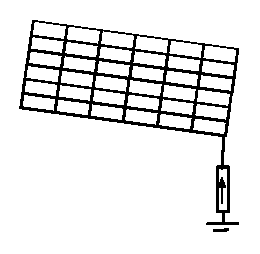
\includegraphics[width=2.9 in]{../resources/image.eps}
		\caption{Equivalent circuit}
	\label{fig:circuitoequivalente}
\end{figure}

Sed posuere consectetur est at lobortis. Maecenas faucibus mollis interdum. Donec id elit non mi porta gravida at eget metus. Donec ullamcorper nulla non metus auctor fringilla. Duis mollis, est non commodo luctus, nisi erat porttitor ligula, eget lacinia odio sem nec elit. Vestibulum id ligula porta felis euismod semper.

Donec ullamcorper nulla non metus auctor fringilla. Cras justo odio, dapibus ac facilisis in, egestas eget quam. Cras mattis consectetur purus sit amet fermentum. Donec sed odio dui.

Vivamus sagittis lacus vel augue laoreet rutrum faucibus dolor auctor. Maecenas faucibus mollis interdum. Nulla vitae elit libero, a pharetra augue. Vestibulum id ligula porta felis euismod semper. Lorem ipsum dolor sit amet, consectetur adipiscing elit.

Cum sociis natoque penatibus et magnis dis parturient montes, nascetur ridiculus mus. Nullam quis risus eget urna mollis ornare vel eu leo. Etiam porta sem malesuada magna mollis euismod. Lorem ipsum dolor sit amet, consectetur adipiscing elit. Praesent commodo cursus magna, vel scelerisque nisl consectetur et.
\begin{align}
	\label{eq:bcurrent}
	\left[\bar{I} \right] = \left[G \right] \cdot \left[ \bar{U} \right]
\end{align}
where $[G]$ is the conductance matrix.

Fusce dapibus, tellus ac cursus commodo, tortor mauris condimentum nibh, ut fermentum massa justo sit amet risus. Aenean lacinia bibendum nulla sed consectetur. Vestibulum id ligula porta felis euismod semper. Donec sed odio dui. Sed posuere consectetur est at lobortis. Curabitur blandit tempus porttitor.

Donec id elit non mi porta gravida at eget metus. Nullam quis risus eget urna mollis ornare vel eu leo. Cum sociis natoque penatibus et magnis dis parturient montes, nascetur ridiculus mus. Sed posuere consectetur est at lobortis. Nulla vitae elit libero, a pharetra augue. Donec sed odio dui. Vivamus sagittis lacus vel augue laoreet rutrum faucibus dolor auctor.
\begin{align}
	\label{eq:full}
	\left[\bar{F} \right] = \left[Y \right] \cdot \left[ \bar{V} \right]
\end{align}
Fusce dapibus, tellus ac cursus commodo, tortor mauris condimentum nibh, ut fermentum massa justo sit amet risus. Aenean lacinia bibendum nulla sed consectetur. Vestibulum id ligula porta felis euismod semper. Donec sed odio dui. Sed posuere consectetur est at lobortis. Curabitur blandit tempus porttitor.

Donec id elit non mi porta gravida at eget metus. Nullam quis risus eget urna mollis ornare vel eu leo. Cum sociis natoque penatibus et magnis dis parturient montes, nascetur ridiculus mus. Sed posuere consectetur est at lobortis. Nulla vitae elit libero, a pharetra augue. Donec sed odio dui. Vivamus sagittis lacus vel augue laoreet rutrum faucibus dolor auctor.
\begin{align}
	\label{eq:biot}
    B=\sum^{r}_{i=0} {\frac{\mu_{0}I_{i}}{4\pi}\int{\frac{\overrightarrow{dl}_{i}\times \overrightarrow{r}_{iP}}{r^{2}_{iP}}}}	
\end{align}

Fusce dapibus, tellus ac cursus commodo, tortor mauris condimentum nibh, ut fermentum massa justo sit amet risus. Aenean lacinia bibendum nulla sed consectetur. Vestibulum id ligula porta felis euismod semper. Donec sed odio dui. Sed posuere consectetur est at lobortis. Curabitur blandit tempus porttitor.

Donec id elit non mi porta gravida at eget metus. Nullam quis risus eget urna mollis ornare vel eu leo. Cum sociis natoque penatibus et magnis dis parturient montes, nascetur ridiculus mus. Sed posuere consectetur est at lobortis. Nulla vitae elit libero, a pharetra augue. Donec sed odio dui. Vivamus sagittis lacus vel augue laoreet rutrum faucibus dolor auctor.

%%FIGURE Substation diagram
\begin{figure}[b]
	\centering
		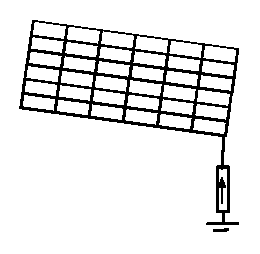
\includegraphics[width=3.5in]{../resources/image.eps}
		\caption{One-line diagram of the substation.}
	\label{fig:substationdiagram}
\end{figure}

\section{Simulated system}

Fusce dapibus, tellus ac cursus commodo, tortor mauris condimentum nibh, ut fermentum massa justo sit amet risus. Aenean lacinia bibendum nulla sed consectetur. Vestibulum id ligula porta felis euismod semper. Donec sed odio dui. Sed posuere consectetur est at lobortis. Curabitur blandit tempus porttitor.

Donec id elit non mi porta gravida at eget metus. Nullam quis risus eget urna mollis ornare vel eu leo. Cum sociis natoque penatibus et magnis dis parturient montes, nascetur ridiculus mus. Sed posuere consectetur est at lobortis. Nulla vitae elit libero, a pharetra augue. Donec sed odio dui. Vivamus sagittis lacus vel augue laoreet rutrum faucibus dolor auctor.

%%FIGURE Substation wire
\begin{figure*}[h]
	\centering
		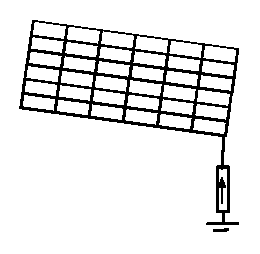
\includegraphics[width=6.1in]{../resources/image.eps}
	\caption{3D wired model of the substation.}
	\label{fig:substationwire}
\end{figure*}

The magnetic field in the substation switchyard was simulated. To do this, both the active conductors and the passive structural elements were modeled using straight line segments with the appropriate sizes and resistivity to reliably represent the real behavior of the conductors.  Specifically, the elements were modeled using conductor segments. The elements used are the following:

\begin{enumerate}
	\item Morbi leo risus, porta ac consectetur ac, vestibulum at eros.
	\item Morbi leo risus, porta ac rty ac, vestibulum at eros.
	\item Morbi leo risus, porta ac rty ac,asdvestibulum at eros.	\item Morbi leo risus, porta ac consectetur rr, vestibulum at eros.
	\item grid.
\end{enumerate}

Fusce dapibus, tellus ac cursus commodo, tortor mauris condimentum nibh, ut fermentum massa justo sit amet risus. Aenean lacinia bibendum nulla sed consectetur. Vestibulum id ligula porta felis euismod semper. Donec sed odio dui. Sed posuere consectetur est at lobortis. Curabitur blandit tempus porttitor.

Donec id elit non mi porta gravida at eget metus. Nullam quis risus eget urna mollis ornare vel eu leo. Cum sociis natoque penatibus et magnis dis parturient montes, nascetur ridiculus mus. Sed posuere consectetur est at lobortis. Nulla vitae elit libero, a pharetra augue. Donec sed odio dui. Vivamus sagittis lacus vel augue laoreet rutrum faucibus dolor auctor.
%%TABLE Table of loads
\begin{table}[bt]
\caption{Load State of the substation.}
		\label{tab:load}
		\centering 
		\small
		\begin{tabular}{c|c|c|c}
		\toprule 
			\textbf{Element} & \textbf{Number} & \textbf{Power $\left[MVA \right]$}	& \textbf{Current $\left[A\right]$} \\ \vgap{1.5pt}
		  \hline \vgap{2.5pt}
			\multirow{5}{*}{Lines} & 1 & 35 & 153.9 \\
			& 2 & 20 & 87.48 \\
			& 3 & 6 & 26.24 \\ 
			& 4 & 16 & 69.98 \\
			& 5 & 40 & 174.95 \\ \hline	\vgap{2.5pt}
			\multirow{6}{*}{Transformers} & \multirow{2}{*} {1} & \multirow{2}{*} {26}  & 1000.74 (LV) \\ & & & 113.72(HV)\\\vgap{2.5pt}
			& \multirow{2}{*} {2} & \multirow{2}{*} {26}  & 1000.74 (LV) \\ & & & 113.72(HV)\\\vgap{2.5pt}
			& \multirow{2}{*} {3} & \multirow{2}{*} {21}  & 808.28 (LV) \\ & & & 91.85 (HV)\\	\vgap{2.5pt}
		\bottomrule
		\end{tabular}
\end{table}

\section{Model Validation}


%%TABLE Table of instruments
\begin{table}[h]
\caption{Measurement Tools}
		\label{tab:tools}
		\centering 
		\small
		\begin{tabular}{c|c}
		\toprule 
			\textbf{Element} & \textbf{Magnetic Field Analyzer} \\ \vgap{1.5pt}
		  	\hline \vgap{2.5pt}
			\multirow{1}{*}{Model} & Wandel \& Goltermann EFA-300 \\
			\multirow{1}{*}{Sensor Surface} & 100 $cm^2$\\
                    	\multirow{1}{*}{Frequency Range} & 5 $Hz$ to 32 $kHz$\\
			\multirow{1}{*}{Magnetic Field Range} & 100 $nT$ to 32 $mT$\\
			\multirow{1}{*}{Noise Level} & 4 $nT$ (30 $Hz$ to 2 $kHz$)\\
			\multirow{1}{*}{Error Margin} & $\pm$3$\%$ at $\geq$ 40 $nT$ (5 $Hz$ to 2 $kHz$)\\
	      	\vgap{2.5pt}
 		\hline 
		\vgap{2.5pt}
			\textbf{Element} & \textbf{Laser Distance Meter} \\ \vgap{1.5pt}
		  	\hline \vgap{2.5pt}
			\multirow{1}{*}{Model} & Leica Disto \\
			\multirow{1}{*}{Distance Range} & 0.2 $m$ to 200 $m$\\
                    	\multirow{1}{*}{Sensibility} & 1 $mm$\\
			\multirow{2}{*}{Precision} & Typical $\pm$3 $mm$ \\
				& Maximum $\pm$5 $mm$ \\
	      	\vgap{2.5pt}
 		\hline 
		\vgap{2.5pt}
			\textbf{Element} & \textbf{Wheel Distance Meter} \\ \vgap{1.5pt}
		  	\hline \vgap{2.5pt}
			\multirow{1}{*}{Model} & Geo-FENNEL M10 \\
			\multirow{1}{*}{Max. Distance Measured} & 9999.99 $m$\\
                    	\multirow{1}{*}{Sensibility} & 10 $mm$\\
			\multirow{1}{*}{Precision} & $\pm$1 $\%$ \\
	      	\vgap{2.5pt}
		\bottomrule
		\end{tabular}
\end{table}

Lorem ipsum dolor sit amet, consectetur adipiscing elit. Praesent commodo cursus magna, vel scelerisque nisl consectetur et. Vestibulum id ligula porta felis euismod semper. Cras mattis consectetur purus sit amet fermentum. Nullam quis risus eget urna mollis ornare vel eu leo. Integer posuere erat a ante venenatis dapibus posuere velit aliquet.

Maecenas sed diam eget risus varius blandit sit amet non magna. Morbi leo risus, porta ac consectetur ac, vestibulum at eros. Vestibulum id ligula porta felis euismod semper. Maecenas faucibus mollis interdum. Sed posuere consectetur est at lobortis. Nulla vitae elit libero, a pharetra augue. Etiam porta sem malesuada magna mollis euismod.

Integer posuere erat a ante venenatis dapibus posuere velit aliquet. Sed posuere consectetur est at lobortis. Maecenas sed diam eget risus varius blandit sit amet non magna. Praesent commodo cursus magna, vel scelerisque nisl consectetur et.

%%FIGURE Measured profiles
\begin{figure}
	\centering
		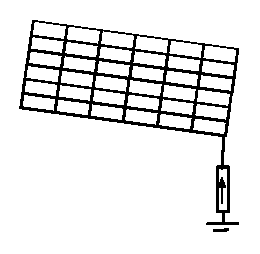
\includegraphics[width=3.5in]{../resources/image.eps}
		\caption{Representation of the measured profiles.}
	\label{fig:slices}
\end{figure}

%%TABLE Measurement profiles endpoints
\begin{table}[!h]
\caption{Measurement profiles endpoints}
		\label{tab:cond}
		\centering 
		\small
		\begin{tabular}{c|c|c|c|c}
			 \toprule 
				\multicolumn{5}{c}{\textbf{Profiles}}  \\ \vgap{1.5pt}
			 \hline \vgap{2.5pt}
			 Points   &  1 &  2 &  3 &  4 \\ \hline \vgap{2.5pt}
			 Initial (x,y) $\left[m \right]$   &  (5,59) &  (-5,0) &  (0,-4.5) &  (79.5,0)\\         			\vgap{1.5pt}
			 Final (x,y) $\left[m \right]$   &  (75,59) &  (-5,55) &  (75,-4.5) &  (79.5,55)\\       
			 \bottomrule
		\end{tabular}
\end{table}

%%TABLE Substation endpoints
\begin{table}[!h]
\caption{Substation endpoints}
		\label{tab:subcoord}
		\centering 
		\small
		\begin{tabular}{c|c|c|c|c}
			 \toprule 
				\multicolumn{5}{c}{\textbf{Substation}}  \\ \vgap{1.5pt}
			 \hline \vgap{2.5pt}
			 Point   &  1 &  2 &  3 &  4 \\ \hline \vgap{2.5pt}
			 Corner (x,y) $\left[m \right]$   &  (5,59) &  (-5,0) &  (0,-4.5) &  (79.5,0)\\         
			 \bottomrule
		\end{tabular}
\end{table}

Lorem ipsum dolor sit amet, consectetur adipiscing elit. Praesent commodo cursus magna, vel scelerisque nisl consectetur et. Vestibulum id ligula porta felis euismod semper. Cras mattis consectetur purus sit amet fermentum. Nullam quis risus eget urna mollis ornare vel eu leo. Integer posuere erat a ante venenatis dapibus posuere velit aliquet.

Maecenas sed diam eget risus varius blandit sit amet non magna. Morbi leo risus, porta ac consectetur ac, vestibulum at eros. Vestibulum id ligula porta felis euismod semper. Maecenas faucibus mollis interdum. Sed posuere consectetur est at lobortis. Nulla vitae elit libero, a pharetra augue. Etiam porta sem malesuada magna mollis euismod.

Integer posuere erat a ante venenatis dapibus posuere velit aliquet. Sed posuere consectetur est at lobortis. Maecenas sed diam eget risus varius blandit sit amet non magna. Praesent commodo cursus magna, vel scelerisque nisl consectetur et.
\begin{figure}[ht]
	\centering
		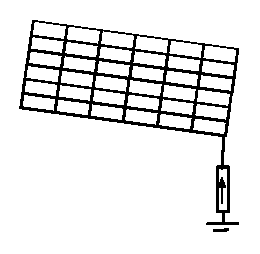
\includegraphics[width=3in]{../resources/image.eps}
		\caption{Simulated and measured magnetic field along profile 1.}
	\label{fig:slice1}
\end{figure}

\begin{figure}[ht]
	\centering
		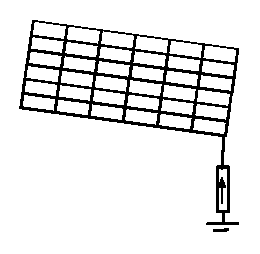
\includegraphics[width=3in]{../resources/image.eps}
		\caption{Simulated and measured magnetic field along profile 2.}
	\label{fig:slice2}
\end{figure}

\begin{figure}[ht]
	\centering
		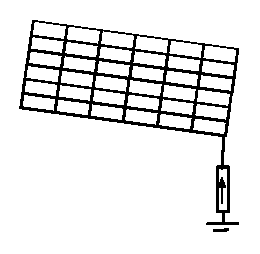
\includegraphics[width=3in]{../resources/image.eps}
		\caption{Simulated and measured magnetic field along profile 3.}
	\label{fig:slice3}
\end{figure}

\begin{figure}[htt]
	\centering
		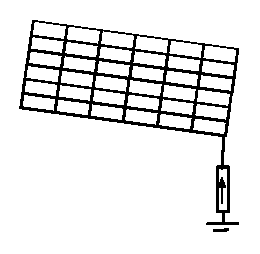
\includegraphics[width=3in]{../resources/image.eps}
		\caption{Simulated and measured magnetic field along profile 4.}
	\label{fig:slice4}
\end{figure}

Lorem ipsum dolor sit amet, consectetur adipiscing elit. Praesent commodo cursus magna, vel scelerisque nisl consectetur et. Vestibulum id ligula porta felis euismod semper. Cras mattis consectetur purus sit amet fermentum. Nullam quis risus eget urna mollis ornare vel eu leo. Integer posuere erat a ante venenatis dapibus posuere velit aliquet.

Maecenas sed diam eget risus varius blandit sit amet non magna. Morbi leo risus, porta ac consectetur ac, vestibulum at eros. Vestibulum id ligula porta felis euismod semper. Maecenas faucibus mollis interdum. Sed posuere consectetur est at lobortis. Nulla vitae elit libero, a pharetra augue. Etiam porta sem malesuada magna mollis euismod.

Integer posuere erat a ante venenatis dapibus posuere velit aliquet. Sed posuere consectetur est at lobortis. Maecenas sed diam eget risus varius blandit sit amet non magna. Praesent commodo cursus magna, vel scelerisque nisl consectetur et.

Some sources of error have been identified, such as:
\begin{itemize}
	\item Aenean lacinia bibendum nulla sed consectetur. Nullam quis risus eget urna mollis ornare vel eu leo.
	\item Aenean lacinia bibendum nulla sed consectetur. Nullam quis risus eget urna mollis ornare vel eu leo.
	\item Aenean lacinia bibendum nulla sed consectetur. Nullam quis risus eget urna mollis ornare vel eu leo.
	\item Aenean lacinia bibendum nulla sed consectetur. Nullam quis risus eget urna mollis ornare vel eu leo.	
	\item IAenean lacinia bibendum nulla sed consectetur. Nullam quis risus eget urna mollis ornare vel eu leo.
\end{itemize}

Aenean lacinia bibendum nulla sed consectetur. Nullam quis risus eget urna mollis ornare vel eu leo.Aenean lacinia bibendum nulla sed consectetur. Nullam quis risus eget urna mollis ornare vel eu leo.
Aenean lacinia bibendum nulla sed consectetur. Nullam quis risus eget urna mollis ornare vel eu leo.

Aenean lacinia bibendum nulla sed consectetur. Nullam quis risus eget urna mollis ornare vel eu leo.

\begin{figure}[!h]
	\centering
		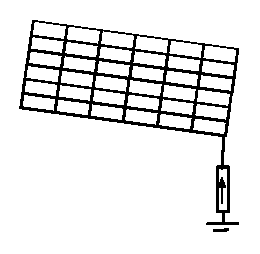
\includegraphics[width=3.4in]{../resources/image.eps}
		\caption{3D plot of the computed magnetic field}
	    \label{fig3wq3:halfs} 
\end{figure}

Vivamus sagittis lacus vel augue laoreet rutrum faucibus dolor auctor. Praesent commodo cursus magna, vel scelerisque nisl consectetur et. Nullam quis risus eget urna mollis ornare vel eu leo. Maecenas faucibus mollis interdum. Vestibulum id ligula porta felis euismod semper.

Duis mollis, est non commodo luctus, nisi erat porttitor ligula, eget lacinia odio sem nec elit. Maecenas sed diam eget risus varius blandit sit amet non magna. Maecenas faucibus mollis interdum. Cras justo odio, dapibus ac facilisis in, egestas eget quam.
\begin{figure}[ht]
	\centering
		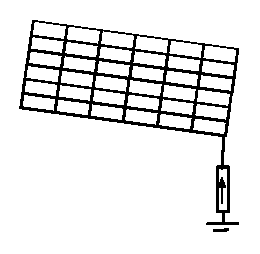
\includegraphics[width=3.5in]{../resources/image.eps}
		\caption{Contour plot of the computed magnetic field.}
	\label{fig:halfsp}
\end{figure}

Vivamus sagittis lacus vel augue laoreet rutrum faucibus dolor auctor. Praesent commodo cursus magna, vel scelerisque nisl consectetur et. Nullam quis risus eget urna mollis ornare vel eu leo. Maecenas faucibus mollis interdum. Vestibulum id ligula porta felis euismod semper.

Duis mollis, est non commodo luctus, nisi erat porttitor ligula, eget lacinia odio sem nec elit. Maecenas sed diam eget risus varius blandit sit amet non magna. Maecenas faucibus mollis interdum. Cras justo odio, dapibus ac facilisis in, egestas eget quam.

Some interesting conclusions could be made from the results regarding the exposure:
\begin{itemize}
	\item Praesent commodo cursus magna, vel scelerisque nisl consectetur et. Aenean lacinia bibendum nulla sed consectetur.
	\item Praesent commodo cursus magna, vel scelerisque nisl consectetur et. Aenean lacinia bibendum nulla sed consectetur.
\end{itemize}

\section{Conclusions}

Vivamus sagittis lacus vel augue laoreet rutrum faucibus dolor auctor. Praesent commodo cursus magna, vel scelerisque nisl consectetur et. Nullam quis risus eget urna mollis ornare vel eu leo. Maecenas faucibus mollis interdum. Vestibulum id ligula porta felis euismod semper.

Duis mollis, est non commodo luctus, nisi erat porttitor ligula, eget lacinia odio sem nec elit. Maecenas sed diam eget risus varius blandit sit amet non magna. Maecenas faucibus mollis interdum. Cras justo odio, dapibus ac facilisis in, egestas eget quam.Vivamus sagittis lacus vel augue laoreet rutrum faucibus dolor auctor. Praesent commodo cursus magna, vel scelerisque nisl consectetur et. Nullam quis risus eget urna mollis ornare vel eu leo. Maecenas faucibus mollis interdum. Vestibulum id ligula porta felis euismod semper.

Duis mollis, est non commodo luctus, nisi erat porttitor ligula, eget lacinia odio sem nec elit. Maecenas sed diam eget risus varius blandit sit amet non magna. Maecenas faucibus mollis interdum. Cras justo odio, dapibus ac facilisis in, egestas eget quam.Vivamus sagittis lacus vel augue laoreet rutrum faucibus dolor auctor. Praesent commodo cursus magna, vel scelerisque nisl consectetur et. Nullam quis risus eget urna mollis ornare vel eu leo. Maecenas faucibus mollis interdum. Vestibulum id ligula porta felis euismod semper.

Duis mollis, est non commodo luctus, nisi erat porttitor ligula, eget lacinia odio sem nec elit. Maecenas sed diam eget risus varius blandit sit amet non magna. Maecenas faucibus mollis interdum. Cras justo odio, dapibus ac facilisis in, egestas eget quam.


\section{Introduction}
\IEEEPARstart{O}{ur} Fusce dapibus, tellus ac cursus commodo, tortor mauris condimentum nibh, ut fermentum massa justo sit amet risus. Morbi leo risus, porta ac consectetur ac, vestibulum at eros. Integer posuere erat a ante venenatis dapibus posuere velit aliquet. Aenean eu leo quam. Pellentesque ornare sem lacinia quam venenatis vestibulum. Curabitur blandit tempus porttitor. Cras justo odio, dapibus ac facilisis in, egestas eget quam.

Aenean eu leo quam. Pellentesque ornare sem lacinia quam venenatis vestibulum. Morbi leo risus, porta ac consectetur ac, vestibulum at eros. Praesent commodo cursus magna, vel scelerisque nisl consectetur et. Maecenas faucibus mollis interdum. Nulla vitae elit libero, a pharetra augue. Lorem ipsum dolor sit amet, consectetur adipiscing elit.

Donec ullamcorper nulla non metus auctor fringilla. Praesent commodo cursus magna, vel scelerisque nisl consectetur et. Nullam quis risus eget urna mollis ornare vel eu leo. Sed posuere consectetur est at lobortis. Fusce dapibus, tellus ac cursus commodo, tortor mauris condimentum nibh, ut fermentum massa justo sit amet risus.

Vivamus sagittis lacus vel augue laoreet rutrum faucibus dolor auctor. Sed posuere consectetur est at lobortis. Maecenas faucibus mollis interdum. Lorem ipsum dolor sit amet, consectetur adipiscing elit. Nullam quis risus eget urna mollis ornare vel eu leo. Vivamus sagittis lacus vel augue laoreet rutrum faucibus dolor auctor.

Sed posuere consectetur est at lobortis. Integer posuere erat a ante venenatis dapibus posuere velit aliquet. Donec id elit non mi porta gravida at eget metus. Morbi leo risus, porta ac consectetur ac, vestibulum at eros. Cras justo odio, dapibus ac facilisis in, egestas eget quam.

Aenean eu leo quam. Pellentesque ornare sem lacinia quam venenatis vestibulum. Morbi leo risus, porta ac consectetur ac, vestibulum at eros. Praesent commodo cursus magna, vel scelerisque nisl consectetur et. Maecenas faucibus mollis interdum. Nulla vitae elit libero, a pharetra augue. Lorem ipsum dolor sit amet, consectetur adipiscing elit.

Donec ullamcorper nulla non metus auctor fringilla. Praesent commodo cursus magna, vel scelerisque nisl consectetur et. Nullam quis risus eget urna mollis ornare vel eu leo. Sed posuere consectetur est at lobortis. Fusce dapibus, tellus ac cursus commodo, tortor mauris condimentum nibh, ut fermentum massa justo sit amet risus.

Vivamus sagittis lacus vel augue laoreet rutrum faucibus dolor auctor. Sed posuere consectetur est at lobortis. Maecenas faucibus mollis interdum. Lorem ipsum dolor sit amet, consectetur adipiscing elit. Nullam quis risus eget urna mollis ornare vel eu leo. Vivamus sagittis lacus vel augue laoreet rutrum faucibus dolor auctor.

Sed posuere consectetur est at lobortis. Integer posuere erat a ante venenatis dapibus posuere velit aliquet. Donec id elit non mi porta gravida at eget metus. Morbi leo risus, porta ac consectetur ac, vestibulum at eros. Cras justo odio, dapibus ac facilisis in, egestas eget quam.

\begin{enumerate}
	\item{Field work.} Sed posuere consectetur est at lobortis. Integer posuere erat a ante venenatis dapibus posuere velit aliquet. Donec id elit non mi porta gravida at eget metus. Morbi leo risus, porta ac consectetur ac, vestibulum at eros. Cras justo odio, dapibus ac facilisis in, egestas eget quam.
	\item{Computer simulation.} Sed posuere consectetur est at lobortis. Integer posuere erat a ante venenatis dapibus posuere velit aliquet. Donec id elit non mi porta gravida at eget metus. Morbi leo risus, porta ac consectetur ac, vestibulum at eros. Cras justo odio, dapibus ac facilisis in, egestas eget quam.
\end{enumerate}

\section{Model description}

Sed posuere consectetur est at lobortis. Integer posuere erat a ante venenatis dapibus posuere velit aliquet. Donec id elit non mi porta gravida at eget metus. Morbi leo risus, porta ac consectetur ac, vestibulum at eros. Cras justo odio, dapibus ac facilisis in, egestas eget quam.

Sed posuere consectetur est at lobortis. Integer posuere erat a ante venenatis dapibus posuere velit aliquet. Donec id elit non mi porta gravida at eget metus. Morbi leo risus, porta ac consectetur ac, vestibulum at eros. Cras justo odio, dapibus ac facilisis in, egestas eget quam.

\begin{enumerate}
	\item Vestibulum id ligula porta felis euismod semper. Aenean eu leo quam. Pellentesque ornare sem lacinia quam venenatis vestibulum.
	\item Vestibulum id ligula porta felis euismod semper. Aenean eu leo quam. Pellentesque ornare sem lacinia quam venenatis vestibulum.
	\item Vestibulum id ligula porta felis euismod semper. Aenean eu leo quam. Pellentesque ornare sem lacinia quam venenatis vestibulum.
\end{enumerate}

Sed posuere consectetur est at lobortis. Maecenas faucibus mollis interdum. Donec id elit non mi porta gravida at eget metus. Donec ullamcorper nulla non metus auctor fringilla. Duis mollis, est non commodo luctus, nisi erat porttitor ligula, eget lacinia odio sem nec elit. Vestibulum id ligula porta felis euismod semper.

Donec ullamcorper nulla non metus auctor fringilla. Cras justo odio, dapibus ac facilisis in, egestas eget quam. Cras mattis consectetur purus sit amet fermentum. Donec sed odio dui.

Vivamus sagittis lacus vel augue laoreet rutrum faucibus dolor auctor. Maecenas faucibus mollis interdum. Nulla vitae elit libero, a pharetra augue. Vestibulum id ligula porta felis euismod semper. Lorem ipsum dolor sit amet, consectetur adipiscing elit.

Cum sociis natoque penatibus et magnis dis parturient montes, nascetur ridiculus mus. Nullam quis risus eget urna mollis ornare vel eu leo. Etiam porta sem malesuada magna mollis euismod. Lorem ipsum dolor sit amet, consectetur adipiscing elit. Praesent commodo cursus magna, vel scelerisque nisl consectetur et.

\begin{figure}[!tb]
	\centering
		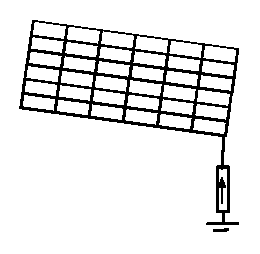
\includegraphics[width=2.9 in]{../resources/image.eps}
		\caption{Equivalent circuit}
	\label{fig:circuitoequivalente}
\end{figure}

Sed posuere consectetur est at lobortis. Maecenas faucibus mollis interdum. Donec id elit non mi porta gravida at eget metus. Donec ullamcorper nulla non metus auctor fringilla. Duis mollis, est non commodo luctus, nisi erat porttitor ligula, eget lacinia odio sem nec elit. Vestibulum id ligula porta felis euismod semper.

Donec ullamcorper nulla non metus auctor fringilla. Cras justo odio, dapibus ac facilisis in, egestas eget quam. Cras mattis consectetur purus sit amet fermentum. Donec sed odio dui.

Vivamus sagittis lacus vel augue laoreet rutrum faucibus dolor auctor. Maecenas faucibus mollis interdum. Nulla vitae elit libero, a pharetra augue. Vestibulum id ligula porta felis euismod semper. Lorem ipsum dolor sit amet, consectetur adipiscing elit.

Cum sociis natoque penatibus et magnis dis parturient montes, nascetur ridiculus mus. Nullam quis risus eget urna mollis ornare vel eu leo. Etiam porta sem malesuada magna mollis euismod. Lorem ipsum dolor sit amet, consectetur adipiscing elit. Praesent commodo cursus magna, vel scelerisque nisl consectetur et.
\begin{align}
	\label{eq:bcurrent}
	\left[\bar{I} \right] = \left[G \right] \cdot \left[ \bar{U} \right]
\end{align}
where $[G]$ is the conductance matrix.

Fusce dapibus, tellus ac cursus commodo, tortor mauris condimentum nibh, ut fermentum massa justo sit amet risus. Aenean lacinia bibendum nulla sed consectetur. Vestibulum id ligula porta felis euismod semper. Donec sed odio dui. Sed posuere consectetur est at lobortis. Curabitur blandit tempus porttitor.

Donec id elit non mi porta gravida at eget metus. Nullam quis risus eget urna mollis ornare vel eu leo. Cum sociis natoque penatibus et magnis dis parturient montes, nascetur ridiculus mus. Sed posuere consectetur est at lobortis. Nulla vitae elit libero, a pharetra augue. Donec sed odio dui. Vivamus sagittis lacus vel augue laoreet rutrum faucibus dolor auctor.
\begin{align}
	\label{eq:full}
	\left[\bar{F} \right] = \left[Y \right] \cdot \left[ \bar{V} \right]
\end{align}
Fusce dapibus, tellus ac cursus commodo, tortor mauris condimentum nibh, ut fermentum massa justo sit amet risus. Aenean lacinia bibendum nulla sed consectetur. Vestibulum id ligula porta felis euismod semper. Donec sed odio dui. Sed posuere consectetur est at lobortis. Curabitur blandit tempus porttitor.

Donec id elit non mi porta gravida at eget metus. Nullam quis risus eget urna mollis ornare vel eu leo. Cum sociis natoque penatibus et magnis dis parturient montes, nascetur ridiculus mus. Sed posuere consectetur est at lobortis. Nulla vitae elit libero, a pharetra augue. Donec sed odio dui. Vivamus sagittis lacus vel augue laoreet rutrum faucibus dolor auctor.
\begin{align}
	\label{eq:biot}
    B=\sum^{r}_{i=0} {\frac{\mu_{0}I_{i}}{4\pi}\int{\frac{\overrightarrow{dl}_{i}\times \overrightarrow{r}_{iP}}{r^{2}_{iP}}}}	
\end{align}

Fusce dapibus, tellus ac cursus commodo, tortor mauris condimentum nibh, ut fermentum massa justo sit amet risus. Aenean lacinia bibendum nulla sed consectetur. Vestibulum id ligula porta felis euismod semper. Donec sed odio dui. Sed posuere consectetur est at lobortis. Curabitur blandit tempus porttitor.

Donec id elit non mi porta gravida at eget metus. Nullam quis risus eget urna mollis ornare vel eu leo. Cum sociis natoque penatibus et magnis dis parturient montes, nascetur ridiculus mus. Sed posuere consectetur est at lobortis. Nulla vitae elit libero, a pharetra augue. Donec sed odio dui. Vivamus sagittis lacus vel augue laoreet rutrum faucibus dolor auctor.

%%FIGURE Substation diagram
\begin{figure}[b]
	\centering
		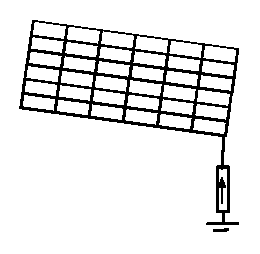
\includegraphics[width=3.5in]{../resources/image.eps}
		\caption{One-line diagram of the substation.}
	\label{fig:substationdiagram}
\end{figure}

\section{Simulated system}

Fusce dapibus, tellus ac cursus commodo, tortor mauris condimentum nibh, ut fermentum massa justo sit amet risus. Aenean lacinia bibendum nulla sed consectetur. Vestibulum id ligula porta felis euismod semper. Donec sed odio dui. Sed posuere consectetur est at lobortis. Curabitur blandit tempus porttitor.

Donec id elit non mi porta gravida at eget metus. Nullam quis risus eget urna mollis ornare vel eu leo. Cum sociis natoque penatibus et magnis dis parturient montes, nascetur ridiculus mus. Sed posuere consectetur est at lobortis. Nulla vitae elit libero, a pharetra augue. Donec sed odio dui. Vivamus sagittis lacus vel augue laoreet rutrum faucibus dolor auctor.

%%FIGURE Substation wire
\begin{figure*}[h]
	\centering
		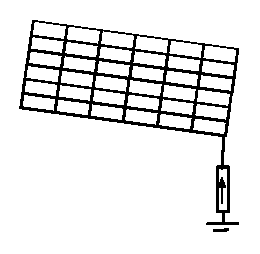
\includegraphics[width=6.1in]{../resources/image.eps}
	\caption{3D wired model of the substation.}
	\label{fig:substationwire}
\end{figure*}

The magnetic field in the substation switchyard was simulated. To do this, both the active conductors and the passive structural elements were modeled using straight line segments with the appropriate sizes and resistivity to reliably represent the real behavior of the conductors.  Specifically, the elements were modeled using conductor segments. The elements used are the following:

\begin{enumerate}
	\item Morbi leo risus, porta ac consectetur ac, vestibulum at eros.
	\item Morbi leo risus, porta ac rty ac, vestibulum at eros.
	\item Morbi leo risus, porta ac rty ac,asdvestibulum at eros.	\item Morbi leo risus, porta ac consectetur rr, vestibulum at eros.
	\item grid.
\end{enumerate}

Fusce dapibus, tellus ac cursus commodo, tortor mauris condimentum nibh, ut fermentum massa justo sit amet risus. Aenean lacinia bibendum nulla sed consectetur. Vestibulum id ligula porta felis euismod semper. Donec sed odio dui. Sed posuere consectetur est at lobortis. Curabitur blandit tempus porttitor.

Donec id elit non mi porta gravida at eget metus. Nullam quis risus eget urna mollis ornare vel eu leo. Cum sociis natoque penatibus et magnis dis parturient montes, nascetur ridiculus mus. Sed posuere consectetur est at lobortis. Nulla vitae elit libero, a pharetra augue. Donec sed odio dui. Vivamus sagittis lacus vel augue laoreet rutrum faucibus dolor auctor.
%%TABLE Table of loads
\begin{table}[bt]
\caption{Load State of the substation.}
		\label{tab:load}
		\centering 
		\small
		\begin{tabular}{c|c|c|c}
		\toprule 
			\textbf{Element} & \textbf{Number} & \textbf{Power $\left[MVA \right]$}	& \textbf{Current $\left[A\right]$} \\ \vgap{1.5pt}
		  \hline \vgap{2.5pt}
			\multirow{5}{*}{Lines} & 1 & 35 & 153.9 \\
			& 2 & 20 & 87.48 \\
			& 3 & 6 & 26.24 \\ 
			& 4 & 16 & 69.98 \\
			& 5 & 40 & 174.95 \\ \hline	\vgap{2.5pt}
			\multirow{6}{*}{Transformers} & \multirow{2}{*} {1} & \multirow{2}{*} {26}  & 1000.74 (LV) \\ & & & 113.72(HV)\\\vgap{2.5pt}
			& \multirow{2}{*} {2} & \multirow{2}{*} {26}  & 1000.74 (LV) \\ & & & 113.72(HV)\\\vgap{2.5pt}
			& \multirow{2}{*} {3} & \multirow{2}{*} {21}  & 808.28 (LV) \\ & & & 91.85 (HV)\\	\vgap{2.5pt}
		\bottomrule
		\end{tabular}
\end{table}

\section{Model Validation}


%%TABLE Table of instruments
\begin{table}[h]
\caption{Measurement Tools}
		\label{tab:tools}
		\centering 
		\small
		\begin{tabular}{c|c}
		\toprule 
			\textbf{Element} & \textbf{Magnetic Field Analyzer} \\ \vgap{1.5pt}
		  	\hline \vgap{2.5pt}
			\multirow{1}{*}{Model} & Wandel \& Goltermann EFA-300 \\
			\multirow{1}{*}{Sensor Surface} & 100 $cm^2$\\
                    	\multirow{1}{*}{Frequency Range} & 5 $Hz$ to 32 $kHz$\\
			\multirow{1}{*}{Magnetic Field Range} & 100 $nT$ to 32 $mT$\\
			\multirow{1}{*}{Noise Level} & 4 $nT$ (30 $Hz$ to 2 $kHz$)\\
			\multirow{1}{*}{Error Margin} & $\pm$3$\%$ at $\geq$ 40 $nT$ (5 $Hz$ to 2 $kHz$)\\
	      	\vgap{2.5pt}
 		\hline 
		\vgap{2.5pt}
			\textbf{Element} & \textbf{Laser Distance Meter} \\ \vgap{1.5pt}
		  	\hline \vgap{2.5pt}
			\multirow{1}{*}{Model} & Leica Disto \\
			\multirow{1}{*}{Distance Range} & 0.2 $m$ to 200 $m$\\
                    	\multirow{1}{*}{Sensibility} & 1 $mm$\\
			\multirow{2}{*}{Precision} & Typical $\pm$3 $mm$ \\
				& Maximum $\pm$5 $mm$ \\
	      	\vgap{2.5pt}
 		\hline 
		\vgap{2.5pt}
			\textbf{Element} & \textbf{Wheel Distance Meter} \\ \vgap{1.5pt}
		  	\hline \vgap{2.5pt}
			\multirow{1}{*}{Model} & Geo-FENNEL M10 \\
			\multirow{1}{*}{Max. Distance Measured} & 9999.99 $m$\\
                    	\multirow{1}{*}{Sensibility} & 10 $mm$\\
			\multirow{1}{*}{Precision} & $\pm$1 $\%$ \\
	      	\vgap{2.5pt}
		\bottomrule
		\end{tabular}
\end{table}

Lorem ipsum dolor sit amet, consectetur adipiscing elit. Praesent commodo cursus magna, vel scelerisque nisl consectetur et. Vestibulum id ligula porta felis euismod semper. Cras mattis consectetur purus sit amet fermentum. Nullam quis risus eget urna mollis ornare vel eu leo. Integer posuere erat a ante venenatis dapibus posuere velit aliquet.

Maecenas sed diam eget risus varius blandit sit amet non magna. Morbi leo risus, porta ac consectetur ac, vestibulum at eros. Vestibulum id ligula porta felis euismod semper. Maecenas faucibus mollis interdum. Sed posuere consectetur est at lobortis. Nulla vitae elit libero, a pharetra augue. Etiam porta sem malesuada magna mollis euismod.

Integer posuere erat a ante venenatis dapibus posuere velit aliquet. Sed posuere consectetur est at lobortis. Maecenas sed diam eget risus varius blandit sit amet non magna. Praesent commodo cursus magna, vel scelerisque nisl consectetur et.

%%FIGURE Measured profiles
\begin{figure}
	\centering
		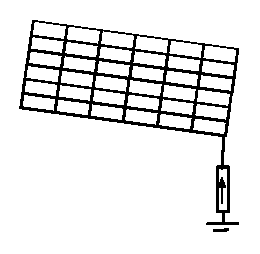
\includegraphics[width=3.5in]{../resources/image.eps}
		\caption{Representation of the measured profiles.}
	\label{fig:slices}
\end{figure}

%%TABLE Measurement profiles endpoints
\begin{table}[!h]
\caption{Measurement profiles endpoints}
		\label{tab:cond}
		\centering 
		\small
		\begin{tabular}{c|c|c|c|c}
			 \toprule 
				\multicolumn{5}{c}{\textbf{Profiles}}  \\ \vgap{1.5pt}
			 \hline \vgap{2.5pt}
			 Points   &  1 &  2 &  3 &  4 \\ \hline \vgap{2.5pt}
			 Initial (x,y) $\left[m \right]$   &  (5,59) &  (-5,0) &  (0,-4.5) &  (79.5,0)\\         			\vgap{1.5pt}
			 Final (x,y) $\left[m \right]$   &  (75,59) &  (-5,55) &  (75,-4.5) &  (79.5,55)\\       
			 \bottomrule
		\end{tabular}
\end{table}

%%TABLE Substation endpoints
\begin{table}[!h]
\caption{Substation endpoints}
		\label{tab:subcoord}
		\centering 
		\small
		\begin{tabular}{c|c|c|c|c}
			 \toprule 
				\multicolumn{5}{c}{\textbf{Substation}}  \\ \vgap{1.5pt}
			 \hline \vgap{2.5pt}
			 Point   &  1 &  2 &  3 &  4 \\ \hline \vgap{2.5pt}
			 Corner (x,y) $\left[m \right]$   &  (5,59) &  (-5,0) &  (0,-4.5) &  (79.5,0)\\         
			 \bottomrule
		\end{tabular}
\end{table}

Lorem ipsum dolor sit amet, consectetur adipiscing elit. Praesent commodo cursus magna, vel scelerisque nisl consectetur et. Vestibulum id ligula porta felis euismod semper. Cras mattis consectetur purus sit amet fermentum. Nullam quis risus eget urna mollis ornare vel eu leo. Integer posuere erat a ante venenatis dapibus posuere velit aliquet.

Maecenas sed diam eget risus varius blandit sit amet non magna. Morbi leo risus, porta ac consectetur ac, vestibulum at eros. Vestibulum id ligula porta felis euismod semper. Maecenas faucibus mollis interdum. Sed posuere consectetur est at lobortis. Nulla vitae elit libero, a pharetra augue. Etiam porta sem malesuada magna mollis euismod.

Integer posuere erat a ante venenatis dapibus posuere velit aliquet. Sed posuere consectetur est at lobortis. Maecenas sed diam eget risus varius blandit sit amet non magna. Praesent commodo cursus magna, vel scelerisque nisl consectetur et.
\begin{figure}[ht]
	\centering
		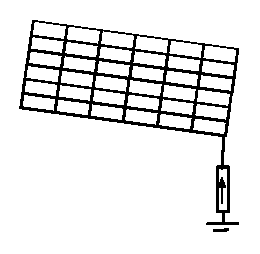
\includegraphics[width=3in]{../resources/image.eps}
		\caption{Simulated and measured magnetic field along profile 1.}
	\label{fig:slice1}
\end{figure}

\begin{figure}[ht]
	\centering
		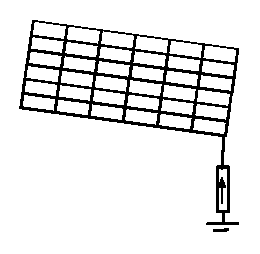
\includegraphics[width=3in]{../resources/image.eps}
		\caption{Simulated and measured magnetic field along profile 2.}
	\label{fig:slice2}
\end{figure}

\begin{figure}[ht]
	\centering
		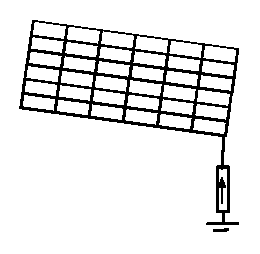
\includegraphics[width=3in]{../resources/image.eps}
		\caption{Simulated and measured magnetic field along profile 3.}
	\label{fig:slice3}
\end{figure}

\begin{figure}[htt]
	\centering
		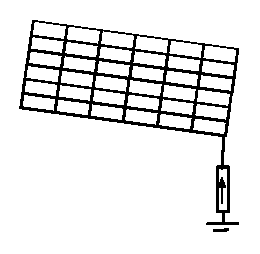
\includegraphics[width=3in]{../resources/image.eps}
		\caption{Simulated and measured magnetic field along profile 4.}
	\label{fig:slice4}
\end{figure}

Lorem ipsum dolor sit amet, consectetur adipiscing elit. Praesent commodo cursus magna, vel scelerisque nisl consectetur et. Vestibulum id ligula porta felis euismod semper. Cras mattis consectetur purus sit amet fermentum. Nullam quis risus eget urna mollis ornare vel eu leo. Integer posuere erat a ante venenatis dapibus posuere velit aliquet.

Maecenas sed diam eget risus varius blandit sit amet non magna. Morbi leo risus, porta ac consectetur ac, vestibulum at eros. Vestibulum id ligula porta felis euismod semper. Maecenas faucibus mollis interdum. Sed posuere consectetur est at lobortis. Nulla vitae elit libero, a pharetra augue. Etiam porta sem malesuada magna mollis euismod.

Integer posuere erat a ante venenatis dapibus posuere velit aliquet. Sed posuere consectetur est at lobortis. Maecenas sed diam eget risus varius blandit sit amet non magna. Praesent commodo cursus magna, vel scelerisque nisl consectetur et.

Some sources of error have been identified, such as:
\begin{itemize}
	\item Aenean lacinia bibendum nulla sed consectetur. Nullam quis risus eget urna mollis ornare vel eu leo.
	\item Aenean lacinia bibendum nulla sed consectetur. Nullam quis risus eget urna mollis ornare vel eu leo.
	\item Aenean lacinia bibendum nulla sed consectetur. Nullam quis risus eget urna mollis ornare vel eu leo.
	\item Aenean lacinia bibendum nulla sed consectetur. Nullam quis risus eget urna mollis ornare vel eu leo.	
	\item IAenean lacinia bibendum nulla sed consectetur. Nullam quis risus eget urna mollis ornare vel eu leo.
\end{itemize}

Aenean lacinia bibendum nulla sed consectetur. Nullam quis risus eget urna mollis ornare vel eu leo.Aenean lacinia bibendum nulla sed consectetur. Nullam quis risus eget urna mollis ornare vel eu leo.
Aenean lacinia bibendum nulla sed consectetur. Nullam quis risus eget urna mollis ornare vel eu leo.

Aenean lacinia bibendum nulla sed consectetur. Nullam quis risus eget urna mollis ornare vel eu leo.

\begin{figure}[!h]
	\centering
		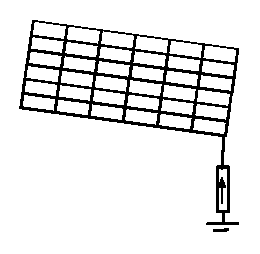
\includegraphics[width=3.4in]{../resources/image.eps}
		\caption{3D plot of the computed magnetic field}
	    \label{fig3wq3:halfs} 
\end{figure}

Vivamus sagittis lacus vel augue laoreet rutrum faucibus dolor auctor. Praesent commodo cursus magna, vel scelerisque nisl consectetur et. Nullam quis risus eget urna mollis ornare vel eu leo. Maecenas faucibus mollis interdum. Vestibulum id ligula porta felis euismod semper.

Duis mollis, est non commodo luctus, nisi erat porttitor ligula, eget lacinia odio sem nec elit. Maecenas sed diam eget risus varius blandit sit amet non magna. Maecenas faucibus mollis interdum. Cras justo odio, dapibus ac facilisis in, egestas eget quam.
\begin{figure}[ht]
	\centering
		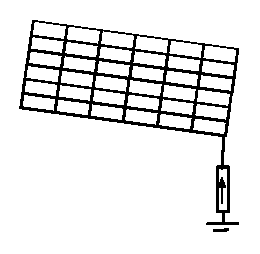
\includegraphics[width=3.5in]{../resources/image.eps}
		\caption{Contour plot of the computed magnetic field.}
	\label{fig:halfsp}
\end{figure}

Vivamus sagittis lacus vel augue laoreet rutrum faucibus dolor auctor. Praesent commodo cursus magna, vel scelerisque nisl consectetur et. Nullam quis risus eget urna mollis ornare vel eu leo. Maecenas faucibus mollis interdum. Vestibulum id ligula porta felis euismod semper.

Duis mollis, est non commodo luctus, nisi erat porttitor ligula, eget lacinia odio sem nec elit. Maecenas sed diam eget risus varius blandit sit amet non magna. Maecenas faucibus mollis interdum. Cras justo odio, dapibus ac facilisis in, egestas eget quam.

Some interesting conclusions could be made from the results regarding the exposure:
\begin{itemize}
	\item Praesent commodo cursus magna, vel scelerisque nisl consectetur et. Aenean lacinia bibendum nulla sed consectetur.
	\item Praesent commodo cursus magna, vel scelerisque nisl consectetur et. Aenean lacinia bibendum nulla sed consectetur.
\end{itemize}

\section{Conclusions}

Vivamus sagittis lacus vel augue laoreet rutrum faucibus dolor auctor. Praesent commodo cursus magna, vel scelerisque nisl consectetur et. Nullam quis risus eget urna mollis ornare vel eu leo. Maecenas faucibus mollis interdum. Vestibulum id ligula porta felis euismod semper.

Duis mollis, est non commodo luctus, nisi erat porttitor ligula, eget lacinia odio sem nec elit. Maecenas sed diam eget risus varius blandit sit amet non magna. Maecenas faucibus mollis interdum. Cras justo odio, dapibus ac facilisis in, egestas eget quam.Vivamus sagittis lacus vel augue laoreet rutrum faucibus dolor auctor. Praesent commodo cursus magna, vel scelerisque nisl consectetur et. Nullam quis risus eget urna mollis ornare vel eu leo. Maecenas faucibus mollis interdum. Vestibulum id ligula porta felis euismod semper.

Duis mollis, est non commodo luctus, nisi erat porttitor ligula, eget lacinia odio sem nec elit. Maecenas sed diam eget risus varius blandit sit amet non magna. Maecenas faucibus mollis interdum. Cras justo odio, dapibus ac facilisis in, egestas eget quam.Vivamus sagittis lacus vel augue laoreet rutrum faucibus dolor auctor. Praesent commodo cursus magna, vel scelerisque nisl consectetur et. Nullam quis risus eget urna mollis ornare vel eu leo. Maecenas faucibus mollis interdum. Vestibulum id ligula porta felis euismod semper.

Duis mollis, est non commodo luctus, nisi erat porttitor ligula, eget lacinia odio sem nec elit. Maecenas sed diam eget risus varius blandit sit amet non magna. Maecenas faucibus mollis interdum. Cras justo odio, dapibus ac facilisis in, egestas eget quam.


\section{Introduction}
\IEEEPARstart{O}{ur} Fusce dapibus, tellus ac cursus commodo, tortor mauris condimentum nibh, ut fermentum massa justo sit amet risus. Morbi leo risus, porta ac consectetur ac, vestibulum at eros. Integer posuere erat a ante venenatis dapibus posuere velit aliquet. Aenean eu leo quam. Pellentesque ornare sem lacinia quam venenatis vestibulum. Curabitur blandit tempus porttitor. Cras justo odio, dapibus ac facilisis in, egestas eget quam.

Aenean eu leo quam. Pellentesque ornare sem lacinia quam venenatis vestibulum. Morbi leo risus, porta ac consectetur ac, vestibulum at eros. Praesent commodo cursus magna, vel scelerisque nisl consectetur et. Maecenas faucibus mollis interdum. Nulla vitae elit libero, a pharetra augue. Lorem ipsum dolor sit amet, consectetur adipiscing elit.

Donec ullamcorper nulla non metus auctor fringilla. Praesent commodo cursus magna, vel scelerisque nisl consectetur et. Nullam quis risus eget urna mollis ornare vel eu leo. Sed posuere consectetur est at lobortis. Fusce dapibus, tellus ac cursus commodo, tortor mauris condimentum nibh, ut fermentum massa justo sit amet risus.

Vivamus sagittis lacus vel augue laoreet rutrum faucibus dolor auctor. Sed posuere consectetur est at lobortis. Maecenas faucibus mollis interdum. Lorem ipsum dolor sit amet, consectetur adipiscing elit. Nullam quis risus eget urna mollis ornare vel eu leo. Vivamus sagittis lacus vel augue laoreet rutrum faucibus dolor auctor.

Sed posuere consectetur est at lobortis. Integer posuere erat a ante venenatis dapibus posuere velit aliquet. Donec id elit non mi porta gravida at eget metus. Morbi leo risus, porta ac consectetur ac, vestibulum at eros. Cras justo odio, dapibus ac facilisis in, egestas eget quam.

Aenean eu leo quam. Pellentesque ornare sem lacinia quam venenatis vestibulum. Morbi leo risus, porta ac consectetur ac, vestibulum at eros. Praesent commodo cursus magna, vel scelerisque nisl consectetur et. Maecenas faucibus mollis interdum. Nulla vitae elit libero, a pharetra augue. Lorem ipsum dolor sit amet, consectetur adipiscing elit.

Donec ullamcorper nulla non metus auctor fringilla. Praesent commodo cursus magna, vel scelerisque nisl consectetur et. Nullam quis risus eget urna mollis ornare vel eu leo. Sed posuere consectetur est at lobortis. Fusce dapibus, tellus ac cursus commodo, tortor mauris condimentum nibh, ut fermentum massa justo sit amet risus.

Vivamus sagittis lacus vel augue laoreet rutrum faucibus dolor auctor. Sed posuere consectetur est at lobortis. Maecenas faucibus mollis interdum. Lorem ipsum dolor sit amet, consectetur adipiscing elit. Nullam quis risus eget urna mollis ornare vel eu leo. Vivamus sagittis lacus vel augue laoreet rutrum faucibus dolor auctor.

Sed posuere consectetur est at lobortis. Integer posuere erat a ante venenatis dapibus posuere velit aliquet. Donec id elit non mi porta gravida at eget metus. Morbi leo risus, porta ac consectetur ac, vestibulum at eros. Cras justo odio, dapibus ac facilisis in, egestas eget quam.

\begin{enumerate}
	\item{Field work.} Sed posuere consectetur est at lobortis. Integer posuere erat a ante venenatis dapibus posuere velit aliquet. Donec id elit non mi porta gravida at eget metus. Morbi leo risus, porta ac consectetur ac, vestibulum at eros. Cras justo odio, dapibus ac facilisis in, egestas eget quam.
	\item{Computer simulation.} Sed posuere consectetur est at lobortis. Integer posuere erat a ante venenatis dapibus posuere velit aliquet. Donec id elit non mi porta gravida at eget metus. Morbi leo risus, porta ac consectetur ac, vestibulum at eros. Cras justo odio, dapibus ac facilisis in, egestas eget quam.
\end{enumerate}

\section{Model description}

Sed posuere consectetur est at lobortis. Integer posuere erat a ante venenatis dapibus posuere velit aliquet. Donec id elit non mi porta gravida at eget metus. Morbi leo risus, porta ac consectetur ac, vestibulum at eros. Cras justo odio, dapibus ac facilisis in, egestas eget quam.

Sed posuere consectetur est at lobortis. Integer posuere erat a ante venenatis dapibus posuere velit aliquet. Donec id elit non mi porta gravida at eget metus. Morbi leo risus, porta ac consectetur ac, vestibulum at eros. Cras justo odio, dapibus ac facilisis in, egestas eget quam.

\begin{enumerate}
	\item Vestibulum id ligula porta felis euismod semper. Aenean eu leo quam. Pellentesque ornare sem lacinia quam venenatis vestibulum.
	\item Vestibulum id ligula porta felis euismod semper. Aenean eu leo quam. Pellentesque ornare sem lacinia quam venenatis vestibulum.
	\item Vestibulum id ligula porta felis euismod semper. Aenean eu leo quam. Pellentesque ornare sem lacinia quam venenatis vestibulum.
\end{enumerate}

Sed posuere consectetur est at lobortis. Maecenas faucibus mollis interdum. Donec id elit non mi porta gravida at eget metus. Donec ullamcorper nulla non metus auctor fringilla. Duis mollis, est non commodo luctus, nisi erat porttitor ligula, eget lacinia odio sem nec elit. Vestibulum id ligula porta felis euismod semper.

Donec ullamcorper nulla non metus auctor fringilla. Cras justo odio, dapibus ac facilisis in, egestas eget quam. Cras mattis consectetur purus sit amet fermentum. Donec sed odio dui.

Vivamus sagittis lacus vel augue laoreet rutrum faucibus dolor auctor. Maecenas faucibus mollis interdum. Nulla vitae elit libero, a pharetra augue. Vestibulum id ligula porta felis euismod semper. Lorem ipsum dolor sit amet, consectetur adipiscing elit.

Cum sociis natoque penatibus et magnis dis parturient montes, nascetur ridiculus mus. Nullam quis risus eget urna mollis ornare vel eu leo. Etiam porta sem malesuada magna mollis euismod. Lorem ipsum dolor sit amet, consectetur adipiscing elit. Praesent commodo cursus magna, vel scelerisque nisl consectetur et.

\begin{figure}[!tb]
	\centering
		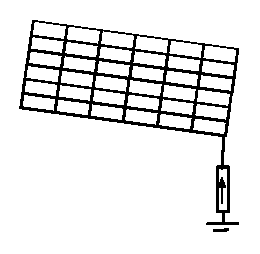
\includegraphics[width=2.9 in]{../resources/image.eps}
		\caption{Equivalent circuit}
	\label{fig:circuitoequivalente}
\end{figure}

Sed posuere consectetur est at lobortis. Maecenas faucibus mollis interdum. Donec id elit non mi porta gravida at eget metus. Donec ullamcorper nulla non metus auctor fringilla. Duis mollis, est non commodo luctus, nisi erat porttitor ligula, eget lacinia odio sem nec elit. Vestibulum id ligula porta felis euismod semper.

Donec ullamcorper nulla non metus auctor fringilla. Cras justo odio, dapibus ac facilisis in, egestas eget quam. Cras mattis consectetur purus sit amet fermentum. Donec sed odio dui.

Vivamus sagittis lacus vel augue laoreet rutrum faucibus dolor auctor. Maecenas faucibus mollis interdum. Nulla vitae elit libero, a pharetra augue. Vestibulum id ligula porta felis euismod semper. Lorem ipsum dolor sit amet, consectetur adipiscing elit.

Cum sociis natoque penatibus et magnis dis parturient montes, nascetur ridiculus mus. Nullam quis risus eget urna mollis ornare vel eu leo. Etiam porta sem malesuada magna mollis euismod. Lorem ipsum dolor sit amet, consectetur adipiscing elit. Praesent commodo cursus magna, vel scelerisque nisl consectetur et.
\begin{align}
	\label{eq:bcurrent}
	\left[\bar{I} \right] = \left[G \right] \cdot \left[ \bar{U} \right]
\end{align}
where $[G]$ is the conductance matrix.

Fusce dapibus, tellus ac cursus commodo, tortor mauris condimentum nibh, ut fermentum massa justo sit amet risus. Aenean lacinia bibendum nulla sed consectetur. Vestibulum id ligula porta felis euismod semper. Donec sed odio dui. Sed posuere consectetur est at lobortis. Curabitur blandit tempus porttitor.

Donec id elit non mi porta gravida at eget metus. Nullam quis risus eget urna mollis ornare vel eu leo. Cum sociis natoque penatibus et magnis dis parturient montes, nascetur ridiculus mus. Sed posuere consectetur est at lobortis. Nulla vitae elit libero, a pharetra augue. Donec sed odio dui. Vivamus sagittis lacus vel augue laoreet rutrum faucibus dolor auctor.
\begin{align}
	\label{eq:full}
	\left[\bar{F} \right] = \left[Y \right] \cdot \left[ \bar{V} \right]
\end{align}
Fusce dapibus, tellus ac cursus commodo, tortor mauris condimentum nibh, ut fermentum massa justo sit amet risus. Aenean lacinia bibendum nulla sed consectetur. Vestibulum id ligula porta felis euismod semper. Donec sed odio dui. Sed posuere consectetur est at lobortis. Curabitur blandit tempus porttitor.

Donec id elit non mi porta gravida at eget metus. Nullam quis risus eget urna mollis ornare vel eu leo. Cum sociis natoque penatibus et magnis dis parturient montes, nascetur ridiculus mus. Sed posuere consectetur est at lobortis. Nulla vitae elit libero, a pharetra augue. Donec sed odio dui. Vivamus sagittis lacus vel augue laoreet rutrum faucibus dolor auctor.
\begin{align}
	\label{eq:biot}
    B=\sum^{r}_{i=0} {\frac{\mu_{0}I_{i}}{4\pi}\int{\frac{\overrightarrow{dl}_{i}\times \overrightarrow{r}_{iP}}{r^{2}_{iP}}}}	
\end{align}

Fusce dapibus, tellus ac cursus commodo, tortor mauris condimentum nibh, ut fermentum massa justo sit amet risus. Aenean lacinia bibendum nulla sed consectetur. Vestibulum id ligula porta felis euismod semper. Donec sed odio dui. Sed posuere consectetur est at lobortis. Curabitur blandit tempus porttitor.

Donec id elit non mi porta gravida at eget metus. Nullam quis risus eget urna mollis ornare vel eu leo. Cum sociis natoque penatibus et magnis dis parturient montes, nascetur ridiculus mus. Sed posuere consectetur est at lobortis. Nulla vitae elit libero, a pharetra augue. Donec sed odio dui. Vivamus sagittis lacus vel augue laoreet rutrum faucibus dolor auctor.

%%FIGURE Substation diagram
\begin{figure}[b]
	\centering
		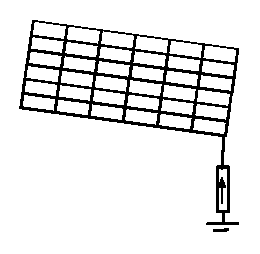
\includegraphics[width=3.5in]{../resources/image.eps}
		\caption{One-line diagram of the substation.}
	\label{fig:substationdiagram}
\end{figure}

\section{Simulated system}

Fusce dapibus, tellus ac cursus commodo, tortor mauris condimentum nibh, ut fermentum massa justo sit amet risus. Aenean lacinia bibendum nulla sed consectetur. Vestibulum id ligula porta felis euismod semper. Donec sed odio dui. Sed posuere consectetur est at lobortis. Curabitur blandit tempus porttitor.

Donec id elit non mi porta gravida at eget metus. Nullam quis risus eget urna mollis ornare vel eu leo. Cum sociis natoque penatibus et magnis dis parturient montes, nascetur ridiculus mus. Sed posuere consectetur est at lobortis. Nulla vitae elit libero, a pharetra augue. Donec sed odio dui. Vivamus sagittis lacus vel augue laoreet rutrum faucibus dolor auctor.

%%FIGURE Substation wire
\begin{figure*}[h]
	\centering
		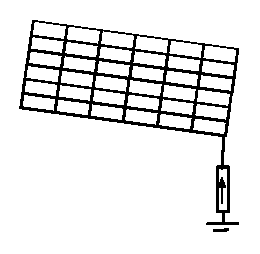
\includegraphics[width=6.1in]{../resources/image.eps}
	\caption{3D wired model of the substation.}
	\label{fig:substationwire}
\end{figure*}

The magnetic field in the substation switchyard was simulated. To do this, both the active conductors and the passive structural elements were modeled using straight line segments with the appropriate sizes and resistivity to reliably represent the real behavior of the conductors.  Specifically, the elements were modeled using conductor segments. The elements used are the following:

\begin{enumerate}
	\item Morbi leo risus, porta ac consectetur ac, vestibulum at eros.
	\item Morbi leo risus, porta ac rty ac, vestibulum at eros.
	\item Morbi leo risus, porta ac rty ac,asdvestibulum at eros.	\item Morbi leo risus, porta ac consectetur rr, vestibulum at eros.
	\item grid.
\end{enumerate}

Fusce dapibus, tellus ac cursus commodo, tortor mauris condimentum nibh, ut fermentum massa justo sit amet risus. Aenean lacinia bibendum nulla sed consectetur. Vestibulum id ligula porta felis euismod semper. Donec sed odio dui. Sed posuere consectetur est at lobortis. Curabitur blandit tempus porttitor.

Donec id elit non mi porta gravida at eget metus. Nullam quis risus eget urna mollis ornare vel eu leo. Cum sociis natoque penatibus et magnis dis parturient montes, nascetur ridiculus mus. Sed posuere consectetur est at lobortis. Nulla vitae elit libero, a pharetra augue. Donec sed odio dui. Vivamus sagittis lacus vel augue laoreet rutrum faucibus dolor auctor.
%%TABLE Table of loads
\begin{table}[bt]
\caption{Load State of the substation.}
		\label{tab:load}
		\centering 
		\small
		\begin{tabular}{c|c|c|c}
		\toprule 
			\textbf{Element} & \textbf{Number} & \textbf{Power $\left[MVA \right]$}	& \textbf{Current $\left[A\right]$} \\ \vgap{1.5pt}
		  \hline \vgap{2.5pt}
			\multirow{5}{*}{Lines} & 1 & 35 & 153.9 \\
			& 2 & 20 & 87.48 \\
			& 3 & 6 & 26.24 \\ 
			& 4 & 16 & 69.98 \\
			& 5 & 40 & 174.95 \\ \hline	\vgap{2.5pt}
			\multirow{6}{*}{Transformers} & \multirow{2}{*} {1} & \multirow{2}{*} {26}  & 1000.74 (LV) \\ & & & 113.72(HV)\\\vgap{2.5pt}
			& \multirow{2}{*} {2} & \multirow{2}{*} {26}  & 1000.74 (LV) \\ & & & 113.72(HV)\\\vgap{2.5pt}
			& \multirow{2}{*} {3} & \multirow{2}{*} {21}  & 808.28 (LV) \\ & & & 91.85 (HV)\\	\vgap{2.5pt}
		\bottomrule
		\end{tabular}
\end{table}

\section{Model Validation}


%%TABLE Table of instruments
\begin{table}[h]
\caption{Measurement Tools}
		\label{tab:tools}
		\centering 
		\small
		\begin{tabular}{c|c}
		\toprule 
			\textbf{Element} & \textbf{Magnetic Field Analyzer} \\ \vgap{1.5pt}
		  	\hline \vgap{2.5pt}
			\multirow{1}{*}{Model} & Wandel \& Goltermann EFA-300 \\
			\multirow{1}{*}{Sensor Surface} & 100 $cm^2$\\
                    	\multirow{1}{*}{Frequency Range} & 5 $Hz$ to 32 $kHz$\\
			\multirow{1}{*}{Magnetic Field Range} & 100 $nT$ to 32 $mT$\\
			\multirow{1}{*}{Noise Level} & 4 $nT$ (30 $Hz$ to 2 $kHz$)\\
			\multirow{1}{*}{Error Margin} & $\pm$3$\%$ at $\geq$ 40 $nT$ (5 $Hz$ to 2 $kHz$)\\
	      	\vgap{2.5pt}
 		\hline 
		\vgap{2.5pt}
			\textbf{Element} & \textbf{Laser Distance Meter} \\ \vgap{1.5pt}
		  	\hline \vgap{2.5pt}
			\multirow{1}{*}{Model} & Leica Disto \\
			\multirow{1}{*}{Distance Range} & 0.2 $m$ to 200 $m$\\
                    	\multirow{1}{*}{Sensibility} & 1 $mm$\\
			\multirow{2}{*}{Precision} & Typical $\pm$3 $mm$ \\
				& Maximum $\pm$5 $mm$ \\
	      	\vgap{2.5pt}
 		\hline 
		\vgap{2.5pt}
			\textbf{Element} & \textbf{Wheel Distance Meter} \\ \vgap{1.5pt}
		  	\hline \vgap{2.5pt}
			\multirow{1}{*}{Model} & Geo-FENNEL M10 \\
			\multirow{1}{*}{Max. Distance Measured} & 9999.99 $m$\\
                    	\multirow{1}{*}{Sensibility} & 10 $mm$\\
			\multirow{1}{*}{Precision} & $\pm$1 $\%$ \\
	      	\vgap{2.5pt}
		\bottomrule
		\end{tabular}
\end{table}

Lorem ipsum dolor sit amet, consectetur adipiscing elit. Praesent commodo cursus magna, vel scelerisque nisl consectetur et. Vestibulum id ligula porta felis euismod semper. Cras mattis consectetur purus sit amet fermentum. Nullam quis risus eget urna mollis ornare vel eu leo. Integer posuere erat a ante venenatis dapibus posuere velit aliquet.

Maecenas sed diam eget risus varius blandit sit amet non magna. Morbi leo risus, porta ac consectetur ac, vestibulum at eros. Vestibulum id ligula porta felis euismod semper. Maecenas faucibus mollis interdum. Sed posuere consectetur est at lobortis. Nulla vitae elit libero, a pharetra augue. Etiam porta sem malesuada magna mollis euismod.

Integer posuere erat a ante venenatis dapibus posuere velit aliquet. Sed posuere consectetur est at lobortis. Maecenas sed diam eget risus varius blandit sit amet non magna. Praesent commodo cursus magna, vel scelerisque nisl consectetur et.

%%FIGURE Measured profiles
\begin{figure}
	\centering
		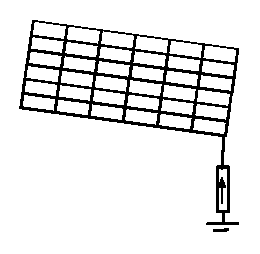
\includegraphics[width=3.5in]{../resources/image.eps}
		\caption{Representation of the measured profiles.}
	\label{fig:slices}
\end{figure}

%%TABLE Measurement profiles endpoints
\begin{table}[!h]
\caption{Measurement profiles endpoints}
		\label{tab:cond}
		\centering 
		\small
		\begin{tabular}{c|c|c|c|c}
			 \toprule 
				\multicolumn{5}{c}{\textbf{Profiles}}  \\ \vgap{1.5pt}
			 \hline \vgap{2.5pt}
			 Points   &  1 &  2 &  3 &  4 \\ \hline \vgap{2.5pt}
			 Initial (x,y) $\left[m \right]$   &  (5,59) &  (-5,0) &  (0,-4.5) &  (79.5,0)\\         			\vgap{1.5pt}
			 Final (x,y) $\left[m \right]$   &  (75,59) &  (-5,55) &  (75,-4.5) &  (79.5,55)\\       
			 \bottomrule
		\end{tabular}
\end{table}

%%TABLE Substation endpoints
\begin{table}[!h]
\caption{Substation endpoints}
		\label{tab:subcoord}
		\centering 
		\small
		\begin{tabular}{c|c|c|c|c}
			 \toprule 
				\multicolumn{5}{c}{\textbf{Substation}}  \\ \vgap{1.5pt}
			 \hline \vgap{2.5pt}
			 Point   &  1 &  2 &  3 &  4 \\ \hline \vgap{2.5pt}
			 Corner (x,y) $\left[m \right]$   &  (5,59) &  (-5,0) &  (0,-4.5) &  (79.5,0)\\         
			 \bottomrule
		\end{tabular}
\end{table}

Lorem ipsum dolor sit amet, consectetur adipiscing elit. Praesent commodo cursus magna, vel scelerisque nisl consectetur et. Vestibulum id ligula porta felis euismod semper. Cras mattis consectetur purus sit amet fermentum. Nullam quis risus eget urna mollis ornare vel eu leo. Integer posuere erat a ante venenatis dapibus posuere velit aliquet.

Maecenas sed diam eget risus varius blandit sit amet non magna. Morbi leo risus, porta ac consectetur ac, vestibulum at eros. Vestibulum id ligula porta felis euismod semper. Maecenas faucibus mollis interdum. Sed posuere consectetur est at lobortis. Nulla vitae elit libero, a pharetra augue. Etiam porta sem malesuada magna mollis euismod.

Integer posuere erat a ante venenatis dapibus posuere velit aliquet. Sed posuere consectetur est at lobortis. Maecenas sed diam eget risus varius blandit sit amet non magna. Praesent commodo cursus magna, vel scelerisque nisl consectetur et.
\begin{figure}[ht]
	\centering
		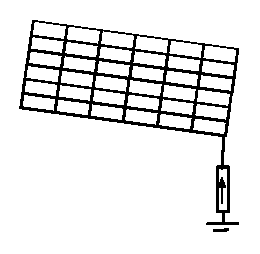
\includegraphics[width=3in]{../resources/image.eps}
		\caption{Simulated and measured magnetic field along profile 1.}
	\label{fig:slice1}
\end{figure}

\begin{figure}[ht]
	\centering
		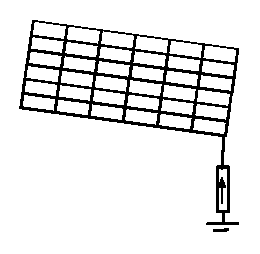
\includegraphics[width=3in]{../resources/image.eps}
		\caption{Simulated and measured magnetic field along profile 2.}
	\label{fig:slice2}
\end{figure}

\begin{figure}[ht]
	\centering
		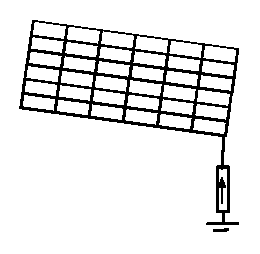
\includegraphics[width=3in]{../resources/image.eps}
		\caption{Simulated and measured magnetic field along profile 3.}
	\label{fig:slice3}
\end{figure}

\begin{figure}[htt]
	\centering
		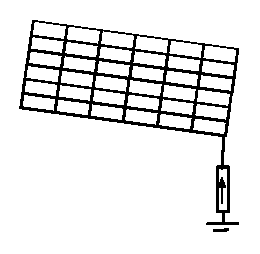
\includegraphics[width=3in]{../resources/image.eps}
		\caption{Simulated and measured magnetic field along profile 4.}
	\label{fig:slice4}
\end{figure}

Lorem ipsum dolor sit amet, consectetur adipiscing elit. Praesent commodo cursus magna, vel scelerisque nisl consectetur et. Vestibulum id ligula porta felis euismod semper. Cras mattis consectetur purus sit amet fermentum. Nullam quis risus eget urna mollis ornare vel eu leo. Integer posuere erat a ante venenatis dapibus posuere velit aliquet.

Maecenas sed diam eget risus varius blandit sit amet non magna. Morbi leo risus, porta ac consectetur ac, vestibulum at eros. Vestibulum id ligula porta felis euismod semper. Maecenas faucibus mollis interdum. Sed posuere consectetur est at lobortis. Nulla vitae elit libero, a pharetra augue. Etiam porta sem malesuada magna mollis euismod.

Integer posuere erat a ante venenatis dapibus posuere velit aliquet. Sed posuere consectetur est at lobortis. Maecenas sed diam eget risus varius blandit sit amet non magna. Praesent commodo cursus magna, vel scelerisque nisl consectetur et.

Some sources of error have been identified, such as:
\begin{itemize}
	\item Aenean lacinia bibendum nulla sed consectetur. Nullam quis risus eget urna mollis ornare vel eu leo.
	\item Aenean lacinia bibendum nulla sed consectetur. Nullam quis risus eget urna mollis ornare vel eu leo.
	\item Aenean lacinia bibendum nulla sed consectetur. Nullam quis risus eget urna mollis ornare vel eu leo.
	\item Aenean lacinia bibendum nulla sed consectetur. Nullam quis risus eget urna mollis ornare vel eu leo.	
	\item IAenean lacinia bibendum nulla sed consectetur. Nullam quis risus eget urna mollis ornare vel eu leo.
\end{itemize}

Aenean lacinia bibendum nulla sed consectetur. Nullam quis risus eget urna mollis ornare vel eu leo.Aenean lacinia bibendum nulla sed consectetur. Nullam quis risus eget urna mollis ornare vel eu leo.
Aenean lacinia bibendum nulla sed consectetur. Nullam quis risus eget urna mollis ornare vel eu leo.

Aenean lacinia bibendum nulla sed consectetur. Nullam quis risus eget urna mollis ornare vel eu leo.

\begin{figure}[!h]
	\centering
		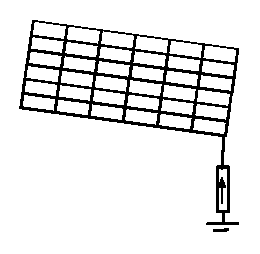
\includegraphics[width=3.4in]{../resources/image.eps}
		\caption{3D plot of the computed magnetic field}
	    \label{fig3wq3:halfs} 
\end{figure}

Vivamus sagittis lacus vel augue laoreet rutrum faucibus dolor auctor. Praesent commodo cursus magna, vel scelerisque nisl consectetur et. Nullam quis risus eget urna mollis ornare vel eu leo. Maecenas faucibus mollis interdum. Vestibulum id ligula porta felis euismod semper.

Duis mollis, est non commodo luctus, nisi erat porttitor ligula, eget lacinia odio sem nec elit. Maecenas sed diam eget risus varius blandit sit amet non magna. Maecenas faucibus mollis interdum. Cras justo odio, dapibus ac facilisis in, egestas eget quam.
\begin{figure}[ht]
	\centering
		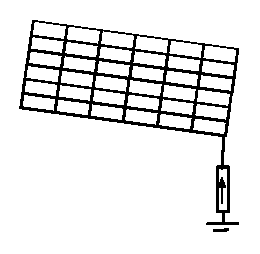
\includegraphics[width=3.5in]{../resources/image.eps}
		\caption{Contour plot of the computed magnetic field.}
	\label{fig:halfsp}
\end{figure}

Vivamus sagittis lacus vel augue laoreet rutrum faucibus dolor auctor. Praesent commodo cursus magna, vel scelerisque nisl consectetur et. Nullam quis risus eget urna mollis ornare vel eu leo. Maecenas faucibus mollis interdum. Vestibulum id ligula porta felis euismod semper.

Duis mollis, est non commodo luctus, nisi erat porttitor ligula, eget lacinia odio sem nec elit. Maecenas sed diam eget risus varius blandit sit amet non magna. Maecenas faucibus mollis interdum. Cras justo odio, dapibus ac facilisis in, egestas eget quam.

Some interesting conclusions could be made from the results regarding the exposure:
\begin{itemize}
	\item Praesent commodo cursus magna, vel scelerisque nisl consectetur et. Aenean lacinia bibendum nulla sed consectetur.
	\item Praesent commodo cursus magna, vel scelerisque nisl consectetur et. Aenean lacinia bibendum nulla sed consectetur.
\end{itemize}

\section{Conclusions}

Vivamus sagittis lacus vel augue laoreet rutrum faucibus dolor auctor. Praesent commodo cursus magna, vel scelerisque nisl consectetur et. Nullam quis risus eget urna mollis ornare vel eu leo. Maecenas faucibus mollis interdum. Vestibulum id ligula porta felis euismod semper.

Duis mollis, est non commodo luctus, nisi erat porttitor ligula, eget lacinia odio sem nec elit. Maecenas sed diam eget risus varius blandit sit amet non magna. Maecenas faucibus mollis interdum. Cras justo odio, dapibus ac facilisis in, egestas eget quam.Vivamus sagittis lacus vel augue laoreet rutrum faucibus dolor auctor. Praesent commodo cursus magna, vel scelerisque nisl consectetur et. Nullam quis risus eget urna mollis ornare vel eu leo. Maecenas faucibus mollis interdum. Vestibulum id ligula porta felis euismod semper.

Duis mollis, est non commodo luctus, nisi erat porttitor ligula, eget lacinia odio sem nec elit. Maecenas sed diam eget risus varius blandit sit amet non magna. Maecenas faucibus mollis interdum. Cras justo odio, dapibus ac facilisis in, egestas eget quam.Vivamus sagittis lacus vel augue laoreet rutrum faucibus dolor auctor. Praesent commodo cursus magna, vel scelerisque nisl consectetur et. Nullam quis risus eget urna mollis ornare vel eu leo. Maecenas faucibus mollis interdum. Vestibulum id ligula porta felis euismod semper.

Duis mollis, est non commodo luctus, nisi erat porttitor ligula, eget lacinia odio sem nec elit. Maecenas sed diam eget risus varius blandit sit amet non magna. Maecenas faucibus mollis interdum. Cras justo odio, dapibus ac facilisis in, egestas eget quam.


\section{Introduction}
\IEEEPARstart{O}{ur} Fusce dapibus, tellus ac cursus commodo, tortor mauris condimentum nibh, ut fermentum massa justo sit amet risus. Morbi leo risus, porta ac consectetur ac, vestibulum at eros. Integer posuere erat a ante venenatis dapibus posuere velit aliquet. Aenean eu leo quam. Pellentesque ornare sem lacinia quam venenatis vestibulum. Curabitur blandit tempus porttitor. Cras justo odio, dapibus ac facilisis in, egestas eget quam.

Aenean eu leo quam. Pellentesque ornare sem lacinia quam venenatis vestibulum. Morbi leo risus, porta ac consectetur ac, vestibulum at eros. Praesent commodo cursus magna, vel scelerisque nisl consectetur et. Maecenas faucibus mollis interdum. Nulla vitae elit libero, a pharetra augue. Lorem ipsum dolor sit amet, consectetur adipiscing elit.

Donec ullamcorper nulla non metus auctor fringilla. Praesent commodo cursus magna, vel scelerisque nisl consectetur et. Nullam quis risus eget urna mollis ornare vel eu leo. Sed posuere consectetur est at lobortis. Fusce dapibus, tellus ac cursus commodo, tortor mauris condimentum nibh, ut fermentum massa justo sit amet risus.

Vivamus sagittis lacus vel augue laoreet rutrum faucibus dolor auctor. Sed posuere consectetur est at lobortis. Maecenas faucibus mollis interdum. Lorem ipsum dolor sit amet, consectetur adipiscing elit. Nullam quis risus eget urna mollis ornare vel eu leo. Vivamus sagittis lacus vel augue laoreet rutrum faucibus dolor auctor.

Sed posuere consectetur est at lobortis. Integer posuere erat a ante venenatis dapibus posuere velit aliquet. Donec id elit non mi porta gravida at eget metus. Morbi leo risus, porta ac consectetur ac, vestibulum at eros. Cras justo odio, dapibus ac facilisis in, egestas eget quam.

Aenean eu leo quam. Pellentesque ornare sem lacinia quam venenatis vestibulum. Morbi leo risus, porta ac consectetur ac, vestibulum at eros. Praesent commodo cursus magna, vel scelerisque nisl consectetur et. Maecenas faucibus mollis interdum. Nulla vitae elit libero, a pharetra augue. Lorem ipsum dolor sit amet, consectetur adipiscing elit.

Donec ullamcorper nulla non metus auctor fringilla. Praesent commodo cursus magna, vel scelerisque nisl consectetur et. Nullam quis risus eget urna mollis ornare vel eu leo. Sed posuere consectetur est at lobortis. Fusce dapibus, tellus ac cursus commodo, tortor mauris condimentum nibh, ut fermentum massa justo sit amet risus.

Vivamus sagittis lacus vel augue laoreet rutrum faucibus dolor auctor. Sed posuere consectetur est at lobortis. Maecenas faucibus mollis interdum. Lorem ipsum dolor sit amet, consectetur adipiscing elit. Nullam quis risus eget urna mollis ornare vel eu leo. Vivamus sagittis lacus vel augue laoreet rutrum faucibus dolor auctor.

Sed posuere consectetur est at lobortis. Integer posuere erat a ante venenatis dapibus posuere velit aliquet. Donec id elit non mi porta gravida at eget metus. Morbi leo risus, porta ac consectetur ac, vestibulum at eros. Cras justo odio, dapibus ac facilisis in, egestas eget quam.

\begin{enumerate}
	\item{Field work.} Sed posuere consectetur est at lobortis. Integer posuere erat a ante venenatis dapibus posuere velit aliquet. Donec id elit non mi porta gravida at eget metus. Morbi leo risus, porta ac consectetur ac, vestibulum at eros. Cras justo odio, dapibus ac facilisis in, egestas eget quam.
	\item{Computer simulation.} Sed posuere consectetur est at lobortis. Integer posuere erat a ante venenatis dapibus posuere velit aliquet. Donec id elit non mi porta gravida at eget metus. Morbi leo risus, porta ac consectetur ac, vestibulum at eros. Cras justo odio, dapibus ac facilisis in, egestas eget quam.
\end{enumerate}

\section{Model description}

Sed posuere consectetur est at lobortis. Integer posuere erat a ante venenatis dapibus posuere velit aliquet. Donec id elit non mi porta gravida at eget metus. Morbi leo risus, porta ac consectetur ac, vestibulum at eros. Cras justo odio, dapibus ac facilisis in, egestas eget quam.

Sed posuere consectetur est at lobortis. Integer posuere erat a ante venenatis dapibus posuere velit aliquet. Donec id elit non mi porta gravida at eget metus. Morbi leo risus, porta ac consectetur ac, vestibulum at eros. Cras justo odio, dapibus ac facilisis in, egestas eget quam.

\begin{enumerate}
	\item Vestibulum id ligula porta felis euismod semper. Aenean eu leo quam. Pellentesque ornare sem lacinia quam venenatis vestibulum.
	\item Vestibulum id ligula porta felis euismod semper. Aenean eu leo quam. Pellentesque ornare sem lacinia quam venenatis vestibulum.
	\item Vestibulum id ligula porta felis euismod semper. Aenean eu leo quam. Pellentesque ornare sem lacinia quam venenatis vestibulum.
\end{enumerate}

Sed posuere consectetur est at lobortis. Maecenas faucibus mollis interdum. Donec id elit non mi porta gravida at eget metus. Donec ullamcorper nulla non metus auctor fringilla. Duis mollis, est non commodo luctus, nisi erat porttitor ligula, eget lacinia odio sem nec elit. Vestibulum id ligula porta felis euismod semper.

Donec ullamcorper nulla non metus auctor fringilla. Cras justo odio, dapibus ac facilisis in, egestas eget quam. Cras mattis consectetur purus sit amet fermentum. Donec sed odio dui.

Vivamus sagittis lacus vel augue laoreet rutrum faucibus dolor auctor. Maecenas faucibus mollis interdum. Nulla vitae elit libero, a pharetra augue. Vestibulum id ligula porta felis euismod semper. Lorem ipsum dolor sit amet, consectetur adipiscing elit.

Cum sociis natoque penatibus et magnis dis parturient montes, nascetur ridiculus mus. Nullam quis risus eget urna mollis ornare vel eu leo. Etiam porta sem malesuada magna mollis euismod. Lorem ipsum dolor sit amet, consectetur adipiscing elit. Praesent commodo cursus magna, vel scelerisque nisl consectetur et.

\begin{figure}[!tb]
	\centering
		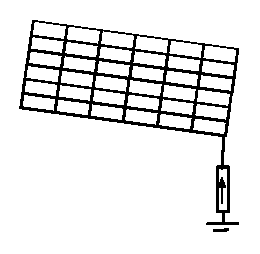
\includegraphics[width=2.9 in]{../resources/image.eps}
		\caption{Equivalent circuit}
	\label{fig:circuitoequivalente}
\end{figure}

Sed posuere consectetur est at lobortis. Maecenas faucibus mollis interdum. Donec id elit non mi porta gravida at eget metus. Donec ullamcorper nulla non metus auctor fringilla. Duis mollis, est non commodo luctus, nisi erat porttitor ligula, eget lacinia odio sem nec elit. Vestibulum id ligula porta felis euismod semper.

Donec ullamcorper nulla non metus auctor fringilla. Cras justo odio, dapibus ac facilisis in, egestas eget quam. Cras mattis consectetur purus sit amet fermentum. Donec sed odio dui.

Vivamus sagittis lacus vel augue laoreet rutrum faucibus dolor auctor. Maecenas faucibus mollis interdum. Nulla vitae elit libero, a pharetra augue. Vestibulum id ligula porta felis euismod semper. Lorem ipsum dolor sit amet, consectetur adipiscing elit.

Cum sociis natoque penatibus et magnis dis parturient montes, nascetur ridiculus mus. Nullam quis risus eget urna mollis ornare vel eu leo. Etiam porta sem malesuada magna mollis euismod. Lorem ipsum dolor sit amet, consectetur adipiscing elit. Praesent commodo cursus magna, vel scelerisque nisl consectetur et.
\begin{align}
	\label{eq:bcurrent}
	\left[\bar{I} \right] = \left[G \right] \cdot \left[ \bar{U} \right]
\end{align}
where $[G]$ is the conductance matrix.

Fusce dapibus, tellus ac cursus commodo, tortor mauris condimentum nibh, ut fermentum massa justo sit amet risus. Aenean lacinia bibendum nulla sed consectetur. Vestibulum id ligula porta felis euismod semper. Donec sed odio dui. Sed posuere consectetur est at lobortis. Curabitur blandit tempus porttitor.

Donec id elit non mi porta gravida at eget metus. Nullam quis risus eget urna mollis ornare vel eu leo. Cum sociis natoque penatibus et magnis dis parturient montes, nascetur ridiculus mus. Sed posuere consectetur est at lobortis. Nulla vitae elit libero, a pharetra augue. Donec sed odio dui. Vivamus sagittis lacus vel augue laoreet rutrum faucibus dolor auctor.
\begin{align}
	\label{eq:full}
	\left[\bar{F} \right] = \left[Y \right] \cdot \left[ \bar{V} \right]
\end{align}
Fusce dapibus, tellus ac cursus commodo, tortor mauris condimentum nibh, ut fermentum massa justo sit amet risus. Aenean lacinia bibendum nulla sed consectetur. Vestibulum id ligula porta felis euismod semper. Donec sed odio dui. Sed posuere consectetur est at lobortis. Curabitur blandit tempus porttitor.

Donec id elit non mi porta gravida at eget metus. Nullam quis risus eget urna mollis ornare vel eu leo. Cum sociis natoque penatibus et magnis dis parturient montes, nascetur ridiculus mus. Sed posuere consectetur est at lobortis. Nulla vitae elit libero, a pharetra augue. Donec sed odio dui. Vivamus sagittis lacus vel augue laoreet rutrum faucibus dolor auctor.
\begin{align}
	\label{eq:biot}
    B=\sum^{r}_{i=0} {\frac{\mu_{0}I_{i}}{4\pi}\int{\frac{\overrightarrow{dl}_{i}\times \overrightarrow{r}_{iP}}{r^{2}_{iP}}}}	
\end{align}

Fusce dapibus, tellus ac cursus commodo, tortor mauris condimentum nibh, ut fermentum massa justo sit amet risus. Aenean lacinia bibendum nulla sed consectetur. Vestibulum id ligula porta felis euismod semper. Donec sed odio dui. Sed posuere consectetur est at lobortis. Curabitur blandit tempus porttitor.

Donec id elit non mi porta gravida at eget metus. Nullam quis risus eget urna mollis ornare vel eu leo. Cum sociis natoque penatibus et magnis dis parturient montes, nascetur ridiculus mus. Sed posuere consectetur est at lobortis. Nulla vitae elit libero, a pharetra augue. Donec sed odio dui. Vivamus sagittis lacus vel augue laoreet rutrum faucibus dolor auctor.

%%FIGURE Substation diagram
\begin{figure}[b]
	\centering
		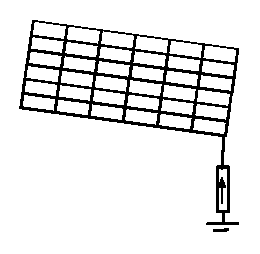
\includegraphics[width=3.5in]{../resources/image.eps}
		\caption{One-line diagram of the substation.}
	\label{fig:substationdiagram}
\end{figure}

\section{Simulated system}

Fusce dapibus, tellus ac cursus commodo, tortor mauris condimentum nibh, ut fermentum massa justo sit amet risus. Aenean lacinia bibendum nulla sed consectetur. Vestibulum id ligula porta felis euismod semper. Donec sed odio dui. Sed posuere consectetur est at lobortis. Curabitur blandit tempus porttitor.

Donec id elit non mi porta gravida at eget metus. Nullam quis risus eget urna mollis ornare vel eu leo. Cum sociis natoque penatibus et magnis dis parturient montes, nascetur ridiculus mus. Sed posuere consectetur est at lobortis. Nulla vitae elit libero, a pharetra augue. Donec sed odio dui. Vivamus sagittis lacus vel augue laoreet rutrum faucibus dolor auctor.

%%FIGURE Substation wire
\begin{figure*}[h]
	\centering
		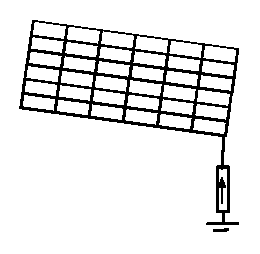
\includegraphics[width=6.1in]{../resources/image.eps}
	\caption{3D wired model of the substation.}
	\label{fig:substationwire}
\end{figure*}

The magnetic field in the substation switchyard was simulated. To do this, both the active conductors and the passive structural elements were modeled using straight line segments with the appropriate sizes and resistivity to reliably represent the real behavior of the conductors.  Specifically, the elements were modeled using conductor segments. The elements used are the following:

\begin{enumerate}
	\item Morbi leo risus, porta ac consectetur ac, vestibulum at eros.
	\item Morbi leo risus, porta ac rty ac, vestibulum at eros.
	\item Morbi leo risus, porta ac rty ac,asdvestibulum at eros.	\item Morbi leo risus, porta ac consectetur rr, vestibulum at eros.
	\item grid.
\end{enumerate}

Fusce dapibus, tellus ac cursus commodo, tortor mauris condimentum nibh, ut fermentum massa justo sit amet risus. Aenean lacinia bibendum nulla sed consectetur. Vestibulum id ligula porta felis euismod semper. Donec sed odio dui. Sed posuere consectetur est at lobortis. Curabitur blandit tempus porttitor.

Donec id elit non mi porta gravida at eget metus. Nullam quis risus eget urna mollis ornare vel eu leo. Cum sociis natoque penatibus et magnis dis parturient montes, nascetur ridiculus mus. Sed posuere consectetur est at lobortis. Nulla vitae elit libero, a pharetra augue. Donec sed odio dui. Vivamus sagittis lacus vel augue laoreet rutrum faucibus dolor auctor.
%%TABLE Table of loads
\begin{table}[bt]
\caption{Load State of the substation.}
		\label{tab:load}
		\centering 
		\small
		\begin{tabular}{c|c|c|c}
		\toprule 
			\textbf{Element} & \textbf{Number} & \textbf{Power $\left[MVA \right]$}	& \textbf{Current $\left[A\right]$} \\ \vgap{1.5pt}
		  \hline \vgap{2.5pt}
			\multirow{5}{*}{Lines} & 1 & 35 & 153.9 \\
			& 2 & 20 & 87.48 \\
			& 3 & 6 & 26.24 \\ 
			& 4 & 16 & 69.98 \\
			& 5 & 40 & 174.95 \\ \hline	\vgap{2.5pt}
			\multirow{6}{*}{Transformers} & \multirow{2}{*} {1} & \multirow{2}{*} {26}  & 1000.74 (LV) \\ & & & 113.72(HV)\\\vgap{2.5pt}
			& \multirow{2}{*} {2} & \multirow{2}{*} {26}  & 1000.74 (LV) \\ & & & 113.72(HV)\\\vgap{2.5pt}
			& \multirow{2}{*} {3} & \multirow{2}{*} {21}  & 808.28 (LV) \\ & & & 91.85 (HV)\\	\vgap{2.5pt}
		\bottomrule
		\end{tabular}
\end{table}

\section{Model Validation}


%%TABLE Table of instruments
\begin{table}[h]
\caption{Measurement Tools}
		\label{tab:tools}
		\centering 
		\small
		\begin{tabular}{c|c}
		\toprule 
			\textbf{Element} & \textbf{Magnetic Field Analyzer} \\ \vgap{1.5pt}
		  	\hline \vgap{2.5pt}
			\multirow{1}{*}{Model} & Wandel \& Goltermann EFA-300 \\
			\multirow{1}{*}{Sensor Surface} & 100 $cm^2$\\
                    	\multirow{1}{*}{Frequency Range} & 5 $Hz$ to 32 $kHz$\\
			\multirow{1}{*}{Magnetic Field Range} & 100 $nT$ to 32 $mT$\\
			\multirow{1}{*}{Noise Level} & 4 $nT$ (30 $Hz$ to 2 $kHz$)\\
			\multirow{1}{*}{Error Margin} & $\pm$3$\%$ at $\geq$ 40 $nT$ (5 $Hz$ to 2 $kHz$)\\
	      	\vgap{2.5pt}
 		\hline 
		\vgap{2.5pt}
			\textbf{Element} & \textbf{Laser Distance Meter} \\ \vgap{1.5pt}
		  	\hline \vgap{2.5pt}
			\multirow{1}{*}{Model} & Leica Disto \\
			\multirow{1}{*}{Distance Range} & 0.2 $m$ to 200 $m$\\
                    	\multirow{1}{*}{Sensibility} & 1 $mm$\\
			\multirow{2}{*}{Precision} & Typical $\pm$3 $mm$ \\
				& Maximum $\pm$5 $mm$ \\
	      	\vgap{2.5pt}
 		\hline 
		\vgap{2.5pt}
			\textbf{Element} & \textbf{Wheel Distance Meter} \\ \vgap{1.5pt}
		  	\hline \vgap{2.5pt}
			\multirow{1}{*}{Model} & Geo-FENNEL M10 \\
			\multirow{1}{*}{Max. Distance Measured} & 9999.99 $m$\\
                    	\multirow{1}{*}{Sensibility} & 10 $mm$\\
			\multirow{1}{*}{Precision} & $\pm$1 $\%$ \\
	      	\vgap{2.5pt}
		\bottomrule
		\end{tabular}
\end{table}

Lorem ipsum dolor sit amet, consectetur adipiscing elit. Praesent commodo cursus magna, vel scelerisque nisl consectetur et. Vestibulum id ligula porta felis euismod semper. Cras mattis consectetur purus sit amet fermentum. Nullam quis risus eget urna mollis ornare vel eu leo. Integer posuere erat a ante venenatis dapibus posuere velit aliquet.

Maecenas sed diam eget risus varius blandit sit amet non magna. Morbi leo risus, porta ac consectetur ac, vestibulum at eros. Vestibulum id ligula porta felis euismod semper. Maecenas faucibus mollis interdum. Sed posuere consectetur est at lobortis. Nulla vitae elit libero, a pharetra augue. Etiam porta sem malesuada magna mollis euismod.

Integer posuere erat a ante venenatis dapibus posuere velit aliquet. Sed posuere consectetur est at lobortis. Maecenas sed diam eget risus varius blandit sit amet non magna. Praesent commodo cursus magna, vel scelerisque nisl consectetur et.

%%FIGURE Measured profiles
\begin{figure}
	\centering
		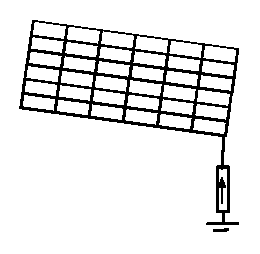
\includegraphics[width=3.5in]{../resources/image.eps}
		\caption{Representation of the measured profiles.}
	\label{fig:slices}
\end{figure}

%%TABLE Measurement profiles endpoints
\begin{table}[!h]
\caption{Measurement profiles endpoints}
		\label{tab:cond}
		\centering 
		\small
		\begin{tabular}{c|c|c|c|c}
			 \toprule 
				\multicolumn{5}{c}{\textbf{Profiles}}  \\ \vgap{1.5pt}
			 \hline \vgap{2.5pt}
			 Points   &  1 &  2 &  3 &  4 \\ \hline \vgap{2.5pt}
			 Initial (x,y) $\left[m \right]$   &  (5,59) &  (-5,0) &  (0,-4.5) &  (79.5,0)\\         			\vgap{1.5pt}
			 Final (x,y) $\left[m \right]$   &  (75,59) &  (-5,55) &  (75,-4.5) &  (79.5,55)\\       
			 \bottomrule
		\end{tabular}
\end{table}

%%TABLE Substation endpoints
\begin{table}[!h]
\caption{Substation endpoints}
		\label{tab:subcoord}
		\centering 
		\small
		\begin{tabular}{c|c|c|c|c}
			 \toprule 
				\multicolumn{5}{c}{\textbf{Substation}}  \\ \vgap{1.5pt}
			 \hline \vgap{2.5pt}
			 Point   &  1 &  2 &  3 &  4 \\ \hline \vgap{2.5pt}
			 Corner (x,y) $\left[m \right]$   &  (5,59) &  (-5,0) &  (0,-4.5) &  (79.5,0)\\         
			 \bottomrule
		\end{tabular}
\end{table}

Lorem ipsum dolor sit amet, consectetur adipiscing elit. Praesent commodo cursus magna, vel scelerisque nisl consectetur et. Vestibulum id ligula porta felis euismod semper. Cras mattis consectetur purus sit amet fermentum. Nullam quis risus eget urna mollis ornare vel eu leo. Integer posuere erat a ante venenatis dapibus posuere velit aliquet.

Maecenas sed diam eget risus varius blandit sit amet non magna. Morbi leo risus, porta ac consectetur ac, vestibulum at eros. Vestibulum id ligula porta felis euismod semper. Maecenas faucibus mollis interdum. Sed posuere consectetur est at lobortis. Nulla vitae elit libero, a pharetra augue. Etiam porta sem malesuada magna mollis euismod.

Integer posuere erat a ante venenatis dapibus posuere velit aliquet. Sed posuere consectetur est at lobortis. Maecenas sed diam eget risus varius blandit sit amet non magna. Praesent commodo cursus magna, vel scelerisque nisl consectetur et.
\begin{figure}[ht]
	\centering
		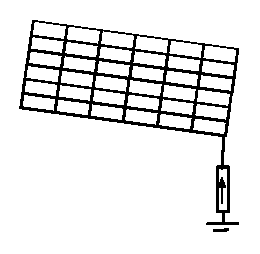
\includegraphics[width=3in]{../resources/image.eps}
		\caption{Simulated and measured magnetic field along profile 1.}
	\label{fig:slice1}
\end{figure}

\begin{figure}[ht]
	\centering
		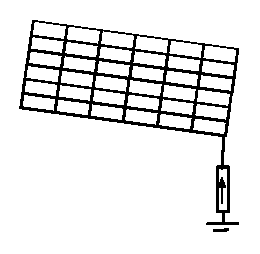
\includegraphics[width=3in]{../resources/image.eps}
		\caption{Simulated and measured magnetic field along profile 2.}
	\label{fig:slice2}
\end{figure}

\begin{figure}[ht]
	\centering
		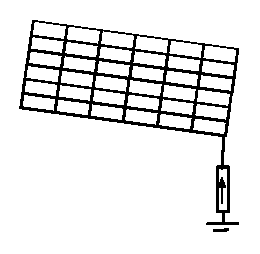
\includegraphics[width=3in]{../resources/image.eps}
		\caption{Simulated and measured magnetic field along profile 3.}
	\label{fig:slice3}
\end{figure}

\begin{figure}[htt]
	\centering
		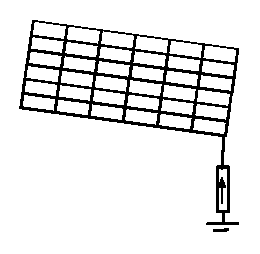
\includegraphics[width=3in]{../resources/image.eps}
		\caption{Simulated and measured magnetic field along profile 4.}
	\label{fig:slice4}
\end{figure}

Lorem ipsum dolor sit amet, consectetur adipiscing elit. Praesent commodo cursus magna, vel scelerisque nisl consectetur et. Vestibulum id ligula porta felis euismod semper. Cras mattis consectetur purus sit amet fermentum. Nullam quis risus eget urna mollis ornare vel eu leo. Integer posuere erat a ante venenatis dapibus posuere velit aliquet.

Maecenas sed diam eget risus varius blandit sit amet non magna. Morbi leo risus, porta ac consectetur ac, vestibulum at eros. Vestibulum id ligula porta felis euismod semper. Maecenas faucibus mollis interdum. Sed posuere consectetur est at lobortis. Nulla vitae elit libero, a pharetra augue. Etiam porta sem malesuada magna mollis euismod.

Integer posuere erat a ante venenatis dapibus posuere velit aliquet. Sed posuere consectetur est at lobortis. Maecenas sed diam eget risus varius blandit sit amet non magna. Praesent commodo cursus magna, vel scelerisque nisl consectetur et.

Some sources of error have been identified, such as:
\begin{itemize}
	\item Aenean lacinia bibendum nulla sed consectetur. Nullam quis risus eget urna mollis ornare vel eu leo.
	\item Aenean lacinia bibendum nulla sed consectetur. Nullam quis risus eget urna mollis ornare vel eu leo.
	\item Aenean lacinia bibendum nulla sed consectetur. Nullam quis risus eget urna mollis ornare vel eu leo.
	\item Aenean lacinia bibendum nulla sed consectetur. Nullam quis risus eget urna mollis ornare vel eu leo.	
	\item IAenean lacinia bibendum nulla sed consectetur. Nullam quis risus eget urna mollis ornare vel eu leo.
\end{itemize}

Aenean lacinia bibendum nulla sed consectetur. Nullam quis risus eget urna mollis ornare vel eu leo.Aenean lacinia bibendum nulla sed consectetur. Nullam quis risus eget urna mollis ornare vel eu leo.
Aenean lacinia bibendum nulla sed consectetur. Nullam quis risus eget urna mollis ornare vel eu leo.

Aenean lacinia bibendum nulla sed consectetur. Nullam quis risus eget urna mollis ornare vel eu leo.

\begin{figure}[!h]
	\centering
		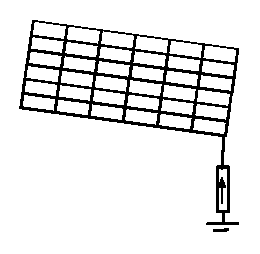
\includegraphics[width=3.4in]{../resources/image.eps}
		\caption{3D plot of the computed magnetic field}
	    \label{fig3wq3:halfs} 
\end{figure}

Vivamus sagittis lacus vel augue laoreet rutrum faucibus dolor auctor. Praesent commodo cursus magna, vel scelerisque nisl consectetur et. Nullam quis risus eget urna mollis ornare vel eu leo. Maecenas faucibus mollis interdum. Vestibulum id ligula porta felis euismod semper.

Duis mollis, est non commodo luctus, nisi erat porttitor ligula, eget lacinia odio sem nec elit. Maecenas sed diam eget risus varius blandit sit amet non magna. Maecenas faucibus mollis interdum. Cras justo odio, dapibus ac facilisis in, egestas eget quam.
\begin{figure}[ht]
	\centering
		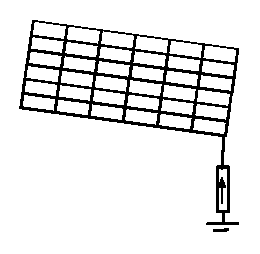
\includegraphics[width=3.5in]{../resources/image.eps}
		\caption{Contour plot of the computed magnetic field.}
	\label{fig:halfsp}
\end{figure}

Vivamus sagittis lacus vel augue laoreet rutrum faucibus dolor auctor. Praesent commodo cursus magna, vel scelerisque nisl consectetur et. Nullam quis risus eget urna mollis ornare vel eu leo. Maecenas faucibus mollis interdum. Vestibulum id ligula porta felis euismod semper.

Duis mollis, est non commodo luctus, nisi erat porttitor ligula, eget lacinia odio sem nec elit. Maecenas sed diam eget risus varius blandit sit amet non magna. Maecenas faucibus mollis interdum. Cras justo odio, dapibus ac facilisis in, egestas eget quam.

Some interesting conclusions could be made from the results regarding the exposure:
\begin{itemize}
	\item Praesent commodo cursus magna, vel scelerisque nisl consectetur et. Aenean lacinia bibendum nulla sed consectetur.
	\item Praesent commodo cursus magna, vel scelerisque nisl consectetur et. Aenean lacinia bibendum nulla sed consectetur.
\end{itemize}

\section{Conclusions}

Vivamus sagittis lacus vel augue laoreet rutrum faucibus dolor auctor. Praesent commodo cursus magna, vel scelerisque nisl consectetur et. Nullam quis risus eget urna mollis ornare vel eu leo. Maecenas faucibus mollis interdum. Vestibulum id ligula porta felis euismod semper.

Duis mollis, est non commodo luctus, nisi erat porttitor ligula, eget lacinia odio sem nec elit. Maecenas sed diam eget risus varius blandit sit amet non magna. Maecenas faucibus mollis interdum. Cras justo odio, dapibus ac facilisis in, egestas eget quam.Vivamus sagittis lacus vel augue laoreet rutrum faucibus dolor auctor. Praesent commodo cursus magna, vel scelerisque nisl consectetur et. Nullam quis risus eget urna mollis ornare vel eu leo. Maecenas faucibus mollis interdum. Vestibulum id ligula porta felis euismod semper.

Duis mollis, est non commodo luctus, nisi erat porttitor ligula, eget lacinia odio sem nec elit. Maecenas sed diam eget risus varius blandit sit amet non magna. Maecenas faucibus mollis interdum. Cras justo odio, dapibus ac facilisis in, egestas eget quam.Vivamus sagittis lacus vel augue laoreet rutrum faucibus dolor auctor. Praesent commodo cursus magna, vel scelerisque nisl consectetur et. Nullam quis risus eget urna mollis ornare vel eu leo. Maecenas faucibus mollis interdum. Vestibulum id ligula porta felis euismod semper.

Duis mollis, est non commodo luctus, nisi erat porttitor ligula, eget lacinia odio sem nec elit. Maecenas sed diam eget risus varius blandit sit amet non magna. Maecenas faucibus mollis interdum. Cras justo odio, dapibus ac facilisis in, egestas eget quam.


\section{Introduction}
\IEEEPARstart{O}{ur} Fusce dapibus, tellus ac cursus commodo, tortor mauris condimentum nibh, ut fermentum massa justo sit amet risus. Morbi leo risus, porta ac consectetur ac, vestibulum at eros. Integer posuere erat a ante venenatis dapibus posuere velit aliquet. Aenean eu leo quam. Pellentesque ornare sem lacinia quam venenatis vestibulum. Curabitur blandit tempus porttitor. Cras justo odio, dapibus ac facilisis in, egestas eget quam.

Aenean eu leo quam. Pellentesque ornare sem lacinia quam venenatis vestibulum. Morbi leo risus, porta ac consectetur ac, vestibulum at eros. Praesent commodo cursus magna, vel scelerisque nisl consectetur et. Maecenas faucibus mollis interdum. Nulla vitae elit libero, a pharetra augue. Lorem ipsum dolor sit amet, consectetur adipiscing elit.

Donec ullamcorper nulla non metus auctor fringilla. Praesent commodo cursus magna, vel scelerisque nisl consectetur et. Nullam quis risus eget urna mollis ornare vel eu leo. Sed posuere consectetur est at lobortis. Fusce dapibus, tellus ac cursus commodo, tortor mauris condimentum nibh, ut fermentum massa justo sit amet risus.

Vivamus sagittis lacus vel augue laoreet rutrum faucibus dolor auctor. Sed posuere consectetur est at lobortis. Maecenas faucibus mollis interdum. Lorem ipsum dolor sit amet, consectetur adipiscing elit. Nullam quis risus eget urna mollis ornare vel eu leo. Vivamus sagittis lacus vel augue laoreet rutrum faucibus dolor auctor.

Sed posuere consectetur est at lobortis. Integer posuere erat a ante venenatis dapibus posuere velit aliquet. Donec id elit non mi porta gravida at eget metus. Morbi leo risus, porta ac consectetur ac, vestibulum at eros. Cras justo odio, dapibus ac facilisis in, egestas eget quam.

Aenean eu leo quam. Pellentesque ornare sem lacinia quam venenatis vestibulum. Morbi leo risus, porta ac consectetur ac, vestibulum at eros. Praesent commodo cursus magna, vel scelerisque nisl consectetur et. Maecenas faucibus mollis interdum. Nulla vitae elit libero, a pharetra augue. Lorem ipsum dolor sit amet, consectetur adipiscing elit.

Donec ullamcorper nulla non metus auctor fringilla. Praesent commodo cursus magna, vel scelerisque nisl consectetur et. Nullam quis risus eget urna mollis ornare vel eu leo. Sed posuere consectetur est at lobortis. Fusce dapibus, tellus ac cursus commodo, tortor mauris condimentum nibh, ut fermentum massa justo sit amet risus.

Vivamus sagittis lacus vel augue laoreet rutrum faucibus dolor auctor. Sed posuere consectetur est at lobortis. Maecenas faucibus mollis interdum. Lorem ipsum dolor sit amet, consectetur adipiscing elit. Nullam quis risus eget urna mollis ornare vel eu leo. Vivamus sagittis lacus vel augue laoreet rutrum faucibus dolor auctor.

Sed posuere consectetur est at lobortis. Integer posuere erat a ante venenatis dapibus posuere velit aliquet. Donec id elit non mi porta gravida at eget metus. Morbi leo risus, porta ac consectetur ac, vestibulum at eros. Cras justo odio, dapibus ac facilisis in, egestas eget quam.

\begin{enumerate}
	\item{Field work.} Sed posuere consectetur est at lobortis. Integer posuere erat a ante venenatis dapibus posuere velit aliquet. Donec id elit non mi porta gravida at eget metus. Morbi leo risus, porta ac consectetur ac, vestibulum at eros. Cras justo odio, dapibus ac facilisis in, egestas eget quam.
	\item{Computer simulation.} Sed posuere consectetur est at lobortis. Integer posuere erat a ante venenatis dapibus posuere velit aliquet. Donec id elit non mi porta gravida at eget metus. Morbi leo risus, porta ac consectetur ac, vestibulum at eros. Cras justo odio, dapibus ac facilisis in, egestas eget quam.
\end{enumerate}

\section{Model description}

Sed posuere consectetur est at lobortis. Integer posuere erat a ante venenatis dapibus posuere velit aliquet. Donec id elit non mi porta gravida at eget metus. Morbi leo risus, porta ac consectetur ac, vestibulum at eros. Cras justo odio, dapibus ac facilisis in, egestas eget quam.

Sed posuere consectetur est at lobortis. Integer posuere erat a ante venenatis dapibus posuere velit aliquet. Donec id elit non mi porta gravida at eget metus. Morbi leo risus, porta ac consectetur ac, vestibulum at eros. Cras justo odio, dapibus ac facilisis in, egestas eget quam.

\begin{enumerate}
	\item Vestibulum id ligula porta felis euismod semper. Aenean eu leo quam. Pellentesque ornare sem lacinia quam venenatis vestibulum.
	\item Vestibulum id ligula porta felis euismod semper. Aenean eu leo quam. Pellentesque ornare sem lacinia quam venenatis vestibulum.
	\item Vestibulum id ligula porta felis euismod semper. Aenean eu leo quam. Pellentesque ornare sem lacinia quam venenatis vestibulum.
\end{enumerate}

Sed posuere consectetur est at lobortis. Maecenas faucibus mollis interdum. Donec id elit non mi porta gravida at eget metus. Donec ullamcorper nulla non metus auctor fringilla. Duis mollis, est non commodo luctus, nisi erat porttitor ligula, eget lacinia odio sem nec elit. Vestibulum id ligula porta felis euismod semper.

Donec ullamcorper nulla non metus auctor fringilla. Cras justo odio, dapibus ac facilisis in, egestas eget quam. Cras mattis consectetur purus sit amet fermentum. Donec sed odio dui.

Vivamus sagittis lacus vel augue laoreet rutrum faucibus dolor auctor. Maecenas faucibus mollis interdum. Nulla vitae elit libero, a pharetra augue. Vestibulum id ligula porta felis euismod semper. Lorem ipsum dolor sit amet, consectetur adipiscing elit.

Cum sociis natoque penatibus et magnis dis parturient montes, nascetur ridiculus mus. Nullam quis risus eget urna mollis ornare vel eu leo. Etiam porta sem malesuada magna mollis euismod. Lorem ipsum dolor sit amet, consectetur adipiscing elit. Praesent commodo cursus magna, vel scelerisque nisl consectetur et.

\begin{figure}[!tb]
	\centering
		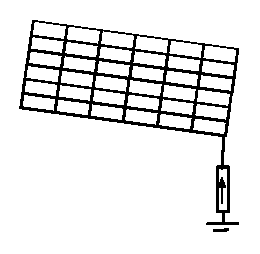
\includegraphics[width=2.9 in]{../resources/image.eps}
		\caption{Equivalent circuit}
	\label{fig:circuitoequivalente}
\end{figure}

Sed posuere consectetur est at lobortis. Maecenas faucibus mollis interdum. Donec id elit non mi porta gravida at eget metus. Donec ullamcorper nulla non metus auctor fringilla. Duis mollis, est non commodo luctus, nisi erat porttitor ligula, eget lacinia odio sem nec elit. Vestibulum id ligula porta felis euismod semper.

Donec ullamcorper nulla non metus auctor fringilla. Cras justo odio, dapibus ac facilisis in, egestas eget quam. Cras mattis consectetur purus sit amet fermentum. Donec sed odio dui.

Vivamus sagittis lacus vel augue laoreet rutrum faucibus dolor auctor. Maecenas faucibus mollis interdum. Nulla vitae elit libero, a pharetra augue. Vestibulum id ligula porta felis euismod semper. Lorem ipsum dolor sit amet, consectetur adipiscing elit.

Cum sociis natoque penatibus et magnis dis parturient montes, nascetur ridiculus mus. Nullam quis risus eget urna mollis ornare vel eu leo. Etiam porta sem malesuada magna mollis euismod. Lorem ipsum dolor sit amet, consectetur adipiscing elit. Praesent commodo cursus magna, vel scelerisque nisl consectetur et.
\begin{align}
	\label{eq:bcurrent}
	\left[\bar{I} \right] = \left[G \right] \cdot \left[ \bar{U} \right]
\end{align}
where $[G]$ is the conductance matrix.

Fusce dapibus, tellus ac cursus commodo, tortor mauris condimentum nibh, ut fermentum massa justo sit amet risus. Aenean lacinia bibendum nulla sed consectetur. Vestibulum id ligula porta felis euismod semper. Donec sed odio dui. Sed posuere consectetur est at lobortis. Curabitur blandit tempus porttitor.

Donec id elit non mi porta gravida at eget metus. Nullam quis risus eget urna mollis ornare vel eu leo. Cum sociis natoque penatibus et magnis dis parturient montes, nascetur ridiculus mus. Sed posuere consectetur est at lobortis. Nulla vitae elit libero, a pharetra augue. Donec sed odio dui. Vivamus sagittis lacus vel augue laoreet rutrum faucibus dolor auctor.
\begin{align}
	\label{eq:full}
	\left[\bar{F} \right] = \left[Y \right] \cdot \left[ \bar{V} \right]
\end{align}
Fusce dapibus, tellus ac cursus commodo, tortor mauris condimentum nibh, ut fermentum massa justo sit amet risus. Aenean lacinia bibendum nulla sed consectetur. Vestibulum id ligula porta felis euismod semper. Donec sed odio dui. Sed posuere consectetur est at lobortis. Curabitur blandit tempus porttitor.

Donec id elit non mi porta gravida at eget metus. Nullam quis risus eget urna mollis ornare vel eu leo. Cum sociis natoque penatibus et magnis dis parturient montes, nascetur ridiculus mus. Sed posuere consectetur est at lobortis. Nulla vitae elit libero, a pharetra augue. Donec sed odio dui. Vivamus sagittis lacus vel augue laoreet rutrum faucibus dolor auctor.
\begin{align}
	\label{eq:biot}
    B=\sum^{r}_{i=0} {\frac{\mu_{0}I_{i}}{4\pi}\int{\frac{\overrightarrow{dl}_{i}\times \overrightarrow{r}_{iP}}{r^{2}_{iP}}}}	
\end{align}

Fusce dapibus, tellus ac cursus commodo, tortor mauris condimentum nibh, ut fermentum massa justo sit amet risus. Aenean lacinia bibendum nulla sed consectetur. Vestibulum id ligula porta felis euismod semper. Donec sed odio dui. Sed posuere consectetur est at lobortis. Curabitur blandit tempus porttitor.

Donec id elit non mi porta gravida at eget metus. Nullam quis risus eget urna mollis ornare vel eu leo. Cum sociis natoque penatibus et magnis dis parturient montes, nascetur ridiculus mus. Sed posuere consectetur est at lobortis. Nulla vitae elit libero, a pharetra augue. Donec sed odio dui. Vivamus sagittis lacus vel augue laoreet rutrum faucibus dolor auctor.

%%FIGURE Substation diagram
\begin{figure}[b]
	\centering
		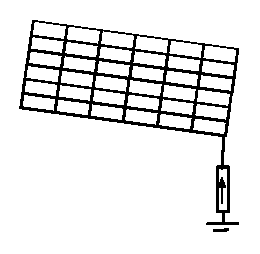
\includegraphics[width=3.5in]{../resources/image.eps}
		\caption{One-line diagram of the substation.}
	\label{fig:substationdiagram}
\end{figure}

\section{Simulated system}

Fusce dapibus, tellus ac cursus commodo, tortor mauris condimentum nibh, ut fermentum massa justo sit amet risus. Aenean lacinia bibendum nulla sed consectetur. Vestibulum id ligula porta felis euismod semper. Donec sed odio dui. Sed posuere consectetur est at lobortis. Curabitur blandit tempus porttitor.

Donec id elit non mi porta gravida at eget metus. Nullam quis risus eget urna mollis ornare vel eu leo. Cum sociis natoque penatibus et magnis dis parturient montes, nascetur ridiculus mus. Sed posuere consectetur est at lobortis. Nulla vitae elit libero, a pharetra augue. Donec sed odio dui. Vivamus sagittis lacus vel augue laoreet rutrum faucibus dolor auctor.

%%FIGURE Substation wire
\begin{figure*}[h]
	\centering
		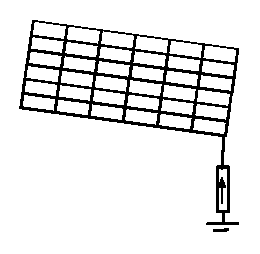
\includegraphics[width=6.1in]{../resources/image.eps}
	\caption{3D wired model of the substation.}
	\label{fig:substationwire}
\end{figure*}

The magnetic field in the substation switchyard was simulated. To do this, both the active conductors and the passive structural elements were modeled using straight line segments with the appropriate sizes and resistivity to reliably represent the real behavior of the conductors.  Specifically, the elements were modeled using conductor segments. The elements used are the following:

\begin{enumerate}
	\item Morbi leo risus, porta ac consectetur ac, vestibulum at eros.
	\item Morbi leo risus, porta ac rty ac, vestibulum at eros.
	\item Morbi leo risus, porta ac rty ac,asdvestibulum at eros.	\item Morbi leo risus, porta ac consectetur rr, vestibulum at eros.
	\item grid.
\end{enumerate}

Fusce dapibus, tellus ac cursus commodo, tortor mauris condimentum nibh, ut fermentum massa justo sit amet risus. Aenean lacinia bibendum nulla sed consectetur. Vestibulum id ligula porta felis euismod semper. Donec sed odio dui. Sed posuere consectetur est at lobortis. Curabitur blandit tempus porttitor.

Donec id elit non mi porta gravida at eget metus. Nullam quis risus eget urna mollis ornare vel eu leo. Cum sociis natoque penatibus et magnis dis parturient montes, nascetur ridiculus mus. Sed posuere consectetur est at lobortis. Nulla vitae elit libero, a pharetra augue. Donec sed odio dui. Vivamus sagittis lacus vel augue laoreet rutrum faucibus dolor auctor.
%%TABLE Table of loads
\begin{table}[bt]
\caption{Load State of the substation.}
		\label{tab:load}
		\centering 
		\small
		\begin{tabular}{c|c|c|c}
		\toprule 
			\textbf{Element} & \textbf{Number} & \textbf{Power $\left[MVA \right]$}	& \textbf{Current $\left[A\right]$} \\ \vgap{1.5pt}
		  \hline \vgap{2.5pt}
			\multirow{5}{*}{Lines} & 1 & 35 & 153.9 \\
			& 2 & 20 & 87.48 \\
			& 3 & 6 & 26.24 \\ 
			& 4 & 16 & 69.98 \\
			& 5 & 40 & 174.95 \\ \hline	\vgap{2.5pt}
			\multirow{6}{*}{Transformers} & \multirow{2}{*} {1} & \multirow{2}{*} {26}  & 1000.74 (LV) \\ & & & 113.72(HV)\\\vgap{2.5pt}
			& \multirow{2}{*} {2} & \multirow{2}{*} {26}  & 1000.74 (LV) \\ & & & 113.72(HV)\\\vgap{2.5pt}
			& \multirow{2}{*} {3} & \multirow{2}{*} {21}  & 808.28 (LV) \\ & & & 91.85 (HV)\\	\vgap{2.5pt}
		\bottomrule
		\end{tabular}
\end{table}

\section{Model Validation}


%%TABLE Table of instruments
\begin{table}[h]
\caption{Measurement Tools}
		\label{tab:tools}
		\centering 
		\small
		\begin{tabular}{c|c}
		\toprule 
			\textbf{Element} & \textbf{Magnetic Field Analyzer} \\ \vgap{1.5pt}
		  	\hline \vgap{2.5pt}
			\multirow{1}{*}{Model} & Wandel \& Goltermann EFA-300 \\
			\multirow{1}{*}{Sensor Surface} & 100 $cm^2$\\
                    	\multirow{1}{*}{Frequency Range} & 5 $Hz$ to 32 $kHz$\\
			\multirow{1}{*}{Magnetic Field Range} & 100 $nT$ to 32 $mT$\\
			\multirow{1}{*}{Noise Level} & 4 $nT$ (30 $Hz$ to 2 $kHz$)\\
			\multirow{1}{*}{Error Margin} & $\pm$3$\%$ at $\geq$ 40 $nT$ (5 $Hz$ to 2 $kHz$)\\
	      	\vgap{2.5pt}
 		\hline 
		\vgap{2.5pt}
			\textbf{Element} & \textbf{Laser Distance Meter} \\ \vgap{1.5pt}
		  	\hline \vgap{2.5pt}
			\multirow{1}{*}{Model} & Leica Disto \\
			\multirow{1}{*}{Distance Range} & 0.2 $m$ to 200 $m$\\
                    	\multirow{1}{*}{Sensibility} & 1 $mm$\\
			\multirow{2}{*}{Precision} & Typical $\pm$3 $mm$ \\
				& Maximum $\pm$5 $mm$ \\
	      	\vgap{2.5pt}
 		\hline 
		\vgap{2.5pt}
			\textbf{Element} & \textbf{Wheel Distance Meter} \\ \vgap{1.5pt}
		  	\hline \vgap{2.5pt}
			\multirow{1}{*}{Model} & Geo-FENNEL M10 \\
			\multirow{1}{*}{Max. Distance Measured} & 9999.99 $m$\\
                    	\multirow{1}{*}{Sensibility} & 10 $mm$\\
			\multirow{1}{*}{Precision} & $\pm$1 $\%$ \\
	      	\vgap{2.5pt}
		\bottomrule
		\end{tabular}
\end{table}

Lorem ipsum dolor sit amet, consectetur adipiscing elit. Praesent commodo cursus magna, vel scelerisque nisl consectetur et. Vestibulum id ligula porta felis euismod semper. Cras mattis consectetur purus sit amet fermentum. Nullam quis risus eget urna mollis ornare vel eu leo. Integer posuere erat a ante venenatis dapibus posuere velit aliquet.

Maecenas sed diam eget risus varius blandit sit amet non magna. Morbi leo risus, porta ac consectetur ac, vestibulum at eros. Vestibulum id ligula porta felis euismod semper. Maecenas faucibus mollis interdum. Sed posuere consectetur est at lobortis. Nulla vitae elit libero, a pharetra augue. Etiam porta sem malesuada magna mollis euismod.

Integer posuere erat a ante venenatis dapibus posuere velit aliquet. Sed posuere consectetur est at lobortis. Maecenas sed diam eget risus varius blandit sit amet non magna. Praesent commodo cursus magna, vel scelerisque nisl consectetur et.

%%FIGURE Measured profiles
\begin{figure}
	\centering
		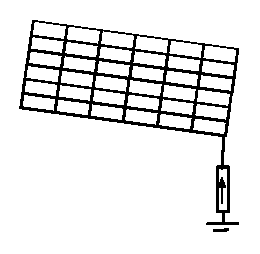
\includegraphics[width=3.5in]{../resources/image.eps}
		\caption{Representation of the measured profiles.}
	\label{fig:slices}
\end{figure}

%%TABLE Measurement profiles endpoints
\begin{table}[!h]
\caption{Measurement profiles endpoints}
		\label{tab:cond}
		\centering 
		\small
		\begin{tabular}{c|c|c|c|c}
			 \toprule 
				\multicolumn{5}{c}{\textbf{Profiles}}  \\ \vgap{1.5pt}
			 \hline \vgap{2.5pt}
			 Points   &  1 &  2 &  3 &  4 \\ \hline \vgap{2.5pt}
			 Initial (x,y) $\left[m \right]$   &  (5,59) &  (-5,0) &  (0,-4.5) &  (79.5,0)\\         			\vgap{1.5pt}
			 Final (x,y) $\left[m \right]$   &  (75,59) &  (-5,55) &  (75,-4.5) &  (79.5,55)\\       
			 \bottomrule
		\end{tabular}
\end{table}

%%TABLE Substation endpoints
\begin{table}[!h]
\caption{Substation endpoints}
		\label{tab:subcoord}
		\centering 
		\small
		\begin{tabular}{c|c|c|c|c}
			 \toprule 
				\multicolumn{5}{c}{\textbf{Substation}}  \\ \vgap{1.5pt}
			 \hline \vgap{2.5pt}
			 Point   &  1 &  2 &  3 &  4 \\ \hline \vgap{2.5pt}
			 Corner (x,y) $\left[m \right]$   &  (5,59) &  (-5,0) &  (0,-4.5) &  (79.5,0)\\         
			 \bottomrule
		\end{tabular}
\end{table}

Lorem ipsum dolor sit amet, consectetur adipiscing elit. Praesent commodo cursus magna, vel scelerisque nisl consectetur et. Vestibulum id ligula porta felis euismod semper. Cras mattis consectetur purus sit amet fermentum. Nullam quis risus eget urna mollis ornare vel eu leo. Integer posuere erat a ante venenatis dapibus posuere velit aliquet.

Maecenas sed diam eget risus varius blandit sit amet non magna. Morbi leo risus, porta ac consectetur ac, vestibulum at eros. Vestibulum id ligula porta felis euismod semper. Maecenas faucibus mollis interdum. Sed posuere consectetur est at lobortis. Nulla vitae elit libero, a pharetra augue. Etiam porta sem malesuada magna mollis euismod.

Integer posuere erat a ante venenatis dapibus posuere velit aliquet. Sed posuere consectetur est at lobortis. Maecenas sed diam eget risus varius blandit sit amet non magna. Praesent commodo cursus magna, vel scelerisque nisl consectetur et.
\begin{figure}[ht]
	\centering
		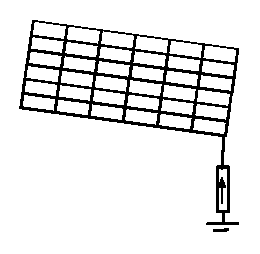
\includegraphics[width=3in]{../resources/image.eps}
		\caption{Simulated and measured magnetic field along profile 1.}
	\label{fig:slice1}
\end{figure}

\begin{figure}[ht]
	\centering
		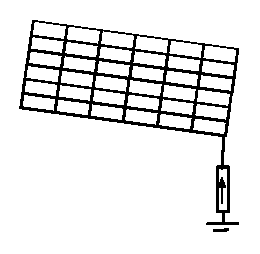
\includegraphics[width=3in]{../resources/image.eps}
		\caption{Simulated and measured magnetic field along profile 2.}
	\label{fig:slice2}
\end{figure}

\begin{figure}[ht]
	\centering
		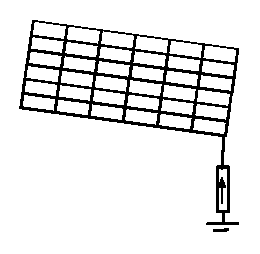
\includegraphics[width=3in]{../resources/image.eps}
		\caption{Simulated and measured magnetic field along profile 3.}
	\label{fig:slice3}
\end{figure}

\begin{figure}[htt]
	\centering
		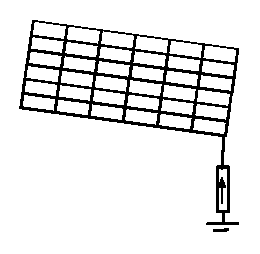
\includegraphics[width=3in]{../resources/image.eps}
		\caption{Simulated and measured magnetic field along profile 4.}
	\label{fig:slice4}
\end{figure}

Lorem ipsum dolor sit amet, consectetur adipiscing elit. Praesent commodo cursus magna, vel scelerisque nisl consectetur et. Vestibulum id ligula porta felis euismod semper. Cras mattis consectetur purus sit amet fermentum. Nullam quis risus eget urna mollis ornare vel eu leo. Integer posuere erat a ante venenatis dapibus posuere velit aliquet.

Maecenas sed diam eget risus varius blandit sit amet non magna. Morbi leo risus, porta ac consectetur ac, vestibulum at eros. Vestibulum id ligula porta felis euismod semper. Maecenas faucibus mollis interdum. Sed posuere consectetur est at lobortis. Nulla vitae elit libero, a pharetra augue. Etiam porta sem malesuada magna mollis euismod.

Integer posuere erat a ante venenatis dapibus posuere velit aliquet. Sed posuere consectetur est at lobortis. Maecenas sed diam eget risus varius blandit sit amet non magna. Praesent commodo cursus magna, vel scelerisque nisl consectetur et.

Some sources of error have been identified, such as:
\begin{itemize}
	\item Aenean lacinia bibendum nulla sed consectetur. Nullam quis risus eget urna mollis ornare vel eu leo.
	\item Aenean lacinia bibendum nulla sed consectetur. Nullam quis risus eget urna mollis ornare vel eu leo.
	\item Aenean lacinia bibendum nulla sed consectetur. Nullam quis risus eget urna mollis ornare vel eu leo.
	\item Aenean lacinia bibendum nulla sed consectetur. Nullam quis risus eget urna mollis ornare vel eu leo.	
	\item IAenean lacinia bibendum nulla sed consectetur. Nullam quis risus eget urna mollis ornare vel eu leo.
\end{itemize}

Aenean lacinia bibendum nulla sed consectetur. Nullam quis risus eget urna mollis ornare vel eu leo.Aenean lacinia bibendum nulla sed consectetur. Nullam quis risus eget urna mollis ornare vel eu leo.
Aenean lacinia bibendum nulla sed consectetur. Nullam quis risus eget urna mollis ornare vel eu leo.

Aenean lacinia bibendum nulla sed consectetur. Nullam quis risus eget urna mollis ornare vel eu leo.

\begin{figure}[!h]
	\centering
		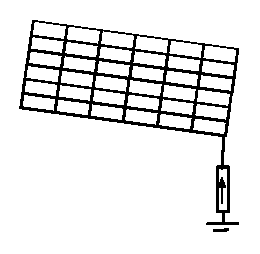
\includegraphics[width=3.4in]{../resources/image.eps}
		\caption{3D plot of the computed magnetic field}
	    \label{fig3wq3:halfs} 
\end{figure}

Vivamus sagittis lacus vel augue laoreet rutrum faucibus dolor auctor. Praesent commodo cursus magna, vel scelerisque nisl consectetur et. Nullam quis risus eget urna mollis ornare vel eu leo. Maecenas faucibus mollis interdum. Vestibulum id ligula porta felis euismod semper.

Duis mollis, est non commodo luctus, nisi erat porttitor ligula, eget lacinia odio sem nec elit. Maecenas sed diam eget risus varius blandit sit amet non magna. Maecenas faucibus mollis interdum. Cras justo odio, dapibus ac facilisis in, egestas eget quam.
\begin{figure}[ht]
	\centering
		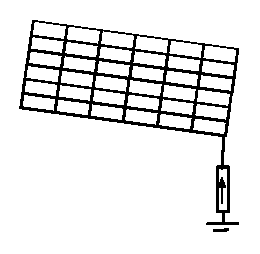
\includegraphics[width=3.5in]{../resources/image.eps}
		\caption{Contour plot of the computed magnetic field.}
	\label{fig:halfsp}
\end{figure}

Vivamus sagittis lacus vel augue laoreet rutrum faucibus dolor auctor. Praesent commodo cursus magna, vel scelerisque nisl consectetur et. Nullam quis risus eget urna mollis ornare vel eu leo. Maecenas faucibus mollis interdum. Vestibulum id ligula porta felis euismod semper.

Duis mollis, est non commodo luctus, nisi erat porttitor ligula, eget lacinia odio sem nec elit. Maecenas sed diam eget risus varius blandit sit amet non magna. Maecenas faucibus mollis interdum. Cras justo odio, dapibus ac facilisis in, egestas eget quam.

Some interesting conclusions could be made from the results regarding the exposure:
\begin{itemize}
	\item Praesent commodo cursus magna, vel scelerisque nisl consectetur et. Aenean lacinia bibendum nulla sed consectetur.
	\item Praesent commodo cursus magna, vel scelerisque nisl consectetur et. Aenean lacinia bibendum nulla sed consectetur.
\end{itemize}

\section{Conclusions}

Vivamus sagittis lacus vel augue laoreet rutrum faucibus dolor auctor. Praesent commodo cursus magna, vel scelerisque nisl consectetur et. Nullam quis risus eget urna mollis ornare vel eu leo. Maecenas faucibus mollis interdum. Vestibulum id ligula porta felis euismod semper.

Duis mollis, est non commodo luctus, nisi erat porttitor ligula, eget lacinia odio sem nec elit. Maecenas sed diam eget risus varius blandit sit amet non magna. Maecenas faucibus mollis interdum. Cras justo odio, dapibus ac facilisis in, egestas eget quam.Vivamus sagittis lacus vel augue laoreet rutrum faucibus dolor auctor. Praesent commodo cursus magna, vel scelerisque nisl consectetur et. Nullam quis risus eget urna mollis ornare vel eu leo. Maecenas faucibus mollis interdum. Vestibulum id ligula porta felis euismod semper.

Duis mollis, est non commodo luctus, nisi erat porttitor ligula, eget lacinia odio sem nec elit. Maecenas sed diam eget risus varius blandit sit amet non magna. Maecenas faucibus mollis interdum. Cras justo odio, dapibus ac facilisis in, egestas eget quam.Vivamus sagittis lacus vel augue laoreet rutrum faucibus dolor auctor. Praesent commodo cursus magna, vel scelerisque nisl consectetur et. Nullam quis risus eget urna mollis ornare vel eu leo. Maecenas faucibus mollis interdum. Vestibulum id ligula porta felis euismod semper.

Duis mollis, est non commodo luctus, nisi erat porttitor ligula, eget lacinia odio sem nec elit. Maecenas sed diam eget risus varius blandit sit amet non magna. Maecenas faucibus mollis interdum. Cras justo odio, dapibus ac facilisis in, egestas eget quam.

\bibliographystyle{IEEEtran}
\bibliography{paperbio}

\vfill

\end{document}
